\documentclass[aspectratio=169,12pt,t]{beamer}

% --- Theme: Metropolis (modern, clean) ---
\usetheme[progressbar=frametitle,numbering=fraction,block=fill]{metropolis}

% --- Fira Sans font (install texlive-fonts-extra if missing) ---
\IfFileExists{FiraSans.sty}{\usepackage[sfdefault]{FiraSans}}{}

% --- Light background with warm accent ---
\definecolor{mDarkTeal}{RGB}{35,55,59}
\definecolor{mLightBrown}{RGB}{235,228,216}
\definecolor{mAccent}{RGB}{140,70,20}

\setbeamercolor{normal text}{fg=mDarkTeal,bg=white}
\setbeamercolor{alerted text}{fg=mAccent}
\setbeamercolor{frametitle}{bg=mDarkTeal,fg=white}
\setbeamercolor{progress bar}{fg=mAccent,bg=mLightBrown}
\setbeamercolor{title separator}{fg=mAccent}
\setbeamercolor{progress bar in head/foot}{fg=mAccent,bg=mLightBrown}
\setbeamercolor{progress bar in section page}{fg=mAccent,bg=mLightBrown}

% --- Packages ---
\usepackage[utf8]{inputenc}
\usepackage{amsmath,amssymb,amsthm}
\usepackage{mathrsfs}
\usepackage{tikz}
\usetikzlibrary{arrows.meta,positioning,calc,decorations.pathreplacing,shapes,patterns}
\usepackage{pgfplots}
\pgfplotsset{compat=1.18}

% --- TikZ diagram styles (shared across the series) ---
\tikzset{
  axisln/.style={-{Stealth[length=2.6mm]}, line width=0.8pt, gray!75},
  curveln/.style={line width=1.6pt, line cap=round, line join=round},
  projln/.style={dash pattern=on 2.6pt off 2pt, line width=0.7pt},
  guide/.style={-{Stealth[length=2.6mm,width=2.2mm]}, line width=1.1pt},
}
% point marker with a white halo: \dotpt{color}{(coord)}
\newcommand{\dotpt}[2]{%
  \fill[white] #2 circle (3.6pt);
  \fill[#1] #2 circle (2.4pt);
}
% open point marker: \opendotpt{color}{(coord)}
\newcommand{\opendotpt}[2]{%
  \fill[white] #2 circle (3.6pt);
  \draw[#1, line width=1pt] #2 circle (2.4pt);
}

% --- Semi-transparent white highlight for text on top of background images ---
\usepackage[most]{tcolorbox}

% Inline highlight: \hl{short text}
\newtcbox{\hl}{%
  nobeforeafter, tcbox raise base,
  colback=white, opacityback=0.6,
  colframe=white, opacityframe=0,
  sharp corners, boxsep=2pt, left=3pt, right=3pt, top=2pt, bottom=2pt%
}

% Block highlight: \begin{hlbox} ... \end{hlbox}  (multi-line, paragraphs, itemize)
% Optional argument accepts any tcolorbox key, e.g. [width=0.6\linewidth]
\newtcolorbox{hlbox}[1][]{%
  enhanced, breakable,
  colback=white, opacityback=0.6,
  colframe=white, opacityframe=0,
  boxsep=3pt, left=6pt, right=6pt, top=4pt, bottom=4pt,
  sharp corners,
  {#1}%
}

% --- Custom colors for content types ---
\definecolor{defcolor}{RGB}{25,85,120}
\definecolor{thmcolor}{RGB}{140,35,35}
\definecolor{proofcolor}{RGB}{35,100,50}
\definecolor{excolor}{RGB}{140,75,10}
\definecolor{remcolor}{RGB}{90,90,90}

% --- Beamer blocks for mathematical content types (semi-transparent) ---
\tcbset{hlblockbase/.style={
  enhanced, breakable,
  coltitle=white, fonttitle=\bfseries,
  opacitybacktitle=0.8, opacityback=0.6,
  opacityframe=0,
  sharp corners,
  boxsep=1pt, left=5pt, right=5pt, top=2pt, bottom=2pt,
  toptitle=1pt, bottomtitle=1pt
}}

\newtcolorbox{defblock}[1]{hlblockbase, title={#1},
  colbacktitle=defcolor, colback=defcolor!15, colframe=defcolor}
\newtcolorbox{thmblock}[1]{hlblockbase, title={#1},
  colbacktitle=thmcolor, colback=thmcolor!15, colframe=thmcolor}
\newtcolorbox{proofblock}[1]{hlblockbase, title={#1},
  colbacktitle=proofcolor, colback=proofcolor!15, colframe=proofcolor}
\newtcolorbox{exblock}[1]{hlblockbase, title={#1},
  colbacktitle=excolor, colback=excolor!15, colframe=excolor}
\newtcolorbox{remblock}[1]{hlblockbase, title={#1},
  colbacktitle=remcolor, colback=remcolor!15, colframe=remcolor}

% --- Metadata ---
\title{Chapter 6: The Riemann--Stieltjes Integral}
\subtitle{Section: Definition and Existence of the Integral}
\author{Based on Walter Rudin's \emph{Principles of Mathematical Analysis}}
\date{}

\begin{document}

{
\usebackgroundtemplate{%
  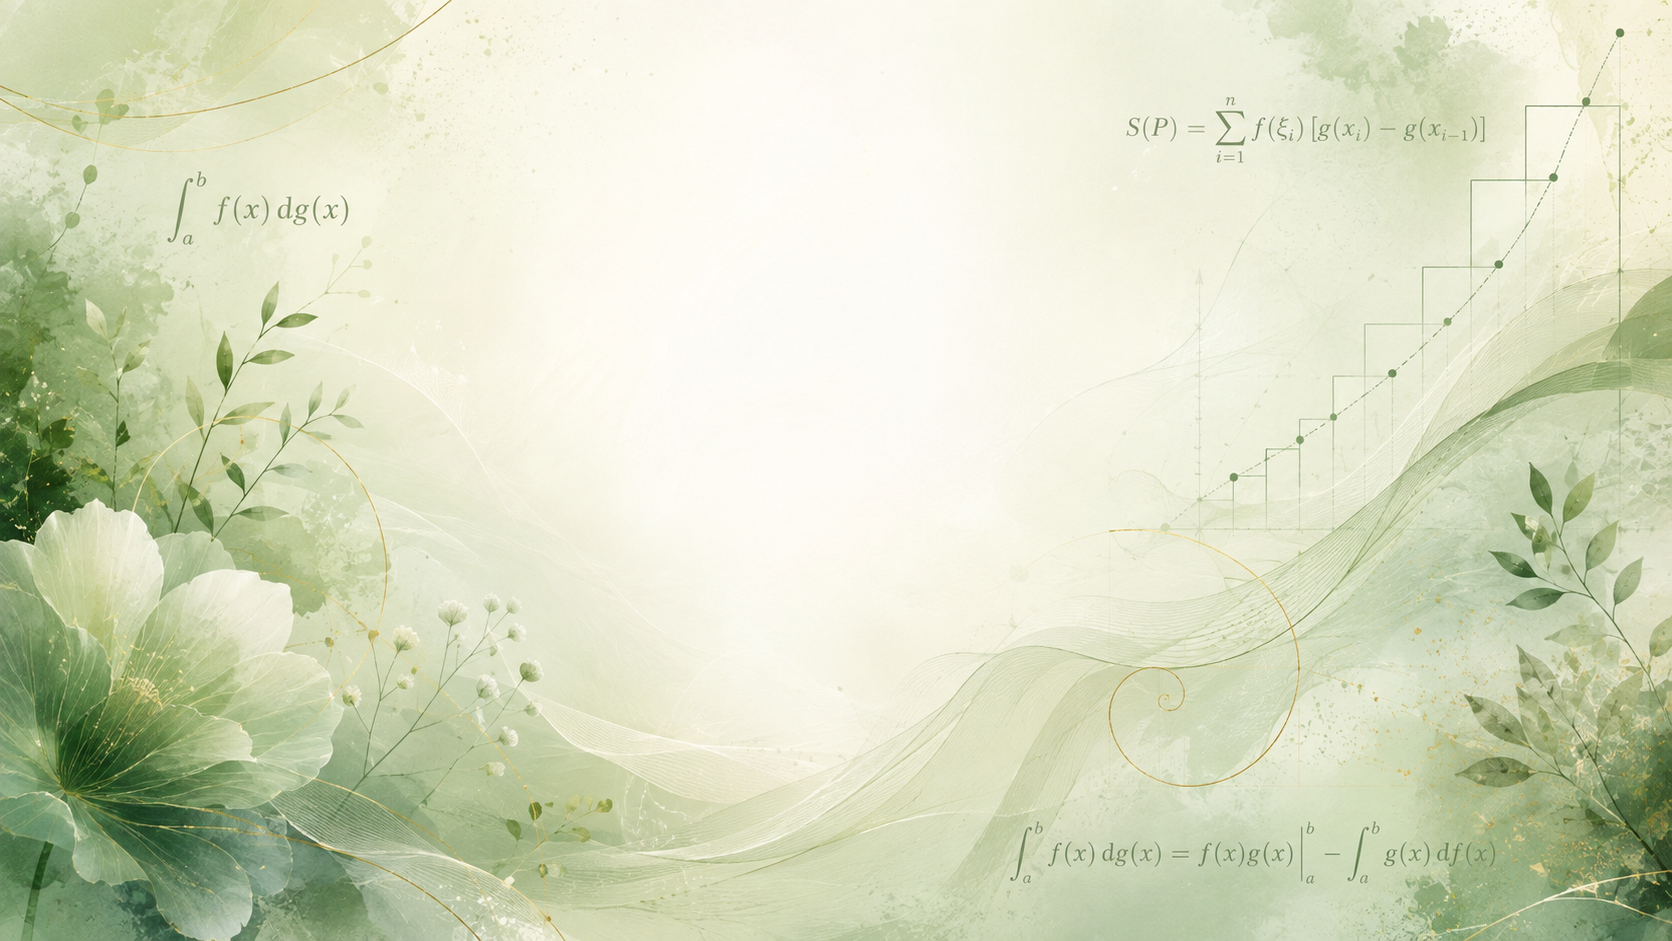
\includegraphics[width=\paperwidth,height=\paperheight,keepaspectratio=false]{chapter_06_bg_00.png}%
}
\begin{frame}[plain]
  \titlepage

  \note{
    Welcome to Chapter 6, Section 1: Definition and Existence of the
    Integral. With this episode we open a brand new chapter and a brand
    new subject: integration. Chapter 5 was about the derivative; now we
    build its partner, the integral, entirely from scratch. Rudin does
    something clever here. Instead of developing only the familiar
    Riemann integral, he immediately introduces a more general object,
    the Riemann-Stieltjes integral, in which a function "f" is
    integrated against a second, monotonically increasing function
    alpha. The ordinary integral becomes the special case where alpha
    of "x" equals "x". In this first section we give the precise
    definitions, prove the basic machinery of refinements, establish
    the fundamental Cauchy-style criterion for integrability, and then
    use it to show that large classes of functions, continuous
    functions in particular, are integrable. Let's get started.
  }
\end{frame}
}

{
\usebackgroundtemplate{%
  
\includegraphics[width=\paperwidth,height=\paperheight,keepaspectratio=false]{chapter_06_bg_01.png}%
}
\begin{frame}[c]{Outline}
  \begin{center}
    \tableofcontents
  \end{center}

  \note{
    Here is the plan for this episode. We begin with motivation: what
    problem the integral solves and why Rudin sets it up through upper
    and lower sums. Then come the two central definitions. Definition
    6.1 constructs the Riemann integral from partitions, and Definition
    6.2 generalizes it to the Riemann-Stieltjes integral, where an
    increasing function alpha acts as a weight. Next we develop the key
    technical tool, refinements of partitions, in Theorems 6.4 and 6.5.
    The heart of the section is Theorem 6.6, a criterion in the style
    of Cauchy that converts integrability into a concrete inequality,
    together with its companion, Theorem 6.7. Finally we harvest the
    consequences: Theorems 6.8 through 6.11 identify large classes of
    integrable functions. We close with a summary and a preview of the
    next episode.
  }
\end{frame}

\section{Motivation}

% --- Build 1/4 ---
\begin{frame}{A New Chapter: Integration}
  \begin{hlbox}
  \begin{itemize}
    \item Chapter 5 built the \alert{derivative}; this chapter builds its
      partner, the \alert{integral}
  \end{itemize}
  \end{hlbox}

  \note{
    Let's set the stage. In Chapter 5 we developed differentiation: the
    local rate of change of a function. This chapter develops the other
    pillar of calculus, integration, which measures a total, an
    accumulated quantity, such as the area under a graph. Throughout
    this chapter we integrate real-valued functions over intervals;
    complex- and vector-valued functions follow in later sections, and
    integration over sets other than intervals must wait for Chapters
    10 and 11. Later in this chapter the derivative and the integral
    will meet in the fundamental theorem of calculus, but first the
    integral has to be defined with full precision.
  }
\end{frame}

% --- Build 2/4 ---
\begin{frame}{A New Chapter: Integration}
  \begin{hlbox}
  \begin{itemize}
    \item Chapter 5 built the \alert{derivative}; this chapter builds its
      partner, the \alert{integral}
    \item The definition rests on the \alert{order structure} of
      $\mathbb{R}$: partitions, suprema, infima --- no limits of sums
      needed
  \end{itemize}
  \end{hlbox}

  \note{
    The construction Rudin chooses depends very explicitly on the order
    structure of the real line. Instead of taking limits of sums as the
    mesh of a partition shrinks, we will trap the integral between
    approximations from above and approximations from below, using
    suprema and infima, the tools we mastered in Chapter 1. This makes
    the theory clean and rigorous with no new limit concepts at all.
  }
\end{frame}

% --- Build 3/4 ---
\begin{frame}{A New Chapter: Integration}
  \begin{hlbox}
  \begin{itemize}
    \item Chapter 5 built the \alert{derivative}; this chapter builds its
      partner, the \alert{integral}
    \item The definition rests on the \alert{order structure} of
      $\mathbb{R}$: partitions, suprema, infima --- no limits of sums
      needed
    \item We generalize immediately: integrate $f$ against an increasing
      \alert{weight} $\alpha$
      \[
        \int_a^b f\,dx \quad\rightsquigarrow\quad \int_a^b f\,d\alpha
        \qquad \text{(Riemann--Stieltjes)}
      \]
  \end{itemize}
  \end{hlbox}

  \note{
    And here is the twist that gives the chapter its name. Almost for
    free, the same construction defines a more general integral, the
    Riemann-Stieltjes integral, written as the integral of "f" with
    respect to alpha. Here alpha is a monotonically increasing function
    that acts as a weight, deciding how much each part of the interval
    counts. Taking alpha of "x" equal to "x" recovers the ordinary
    Riemann integral, so nothing is lost by generalizing, and, as we
    will see in the next episode, a great deal is gained.
  }
\end{frame}

% --- Build 4/4 ---
\begin{frame}{A New Chapter: Integration}
  \begin{hlbox}
  \begin{itemize}
    \item Chapter 5 built the \alert{derivative}; this chapter builds its
      partner, the \alert{integral}
    \item The definition rests on the \alert{order structure} of
      $\mathbb{R}$: partitions, suprema, infima --- no limits of sums
      needed
    \item We generalize immediately: integrate $f$ against an increasing
      \alert{weight} $\alpha$
      \[
        \int_a^b f\,dx \quad\rightsquigarrow\quad \int_a^b f\,d\alpha
        \qquad \text{(Riemann--Stieltjes)}
      \]
    \item Central question: \alert{which functions are integrable?}
  \end{itemize}
  \end{hlbox}

  \note{
    The central question of this section is the last line on the
    slide: for which functions "f" does the integral actually exist?
    The construction will make sense for every bounded "f", but its
    two halves, an estimate from above and an estimate from below,
    need not agree. The main theorems of this episode, Theorems 6.8
    through 6.11, give broad sufficient conditions for agreement.
    Before the formal definitions, let's fix the geometric picture
    that drives everything.
  }
\end{frame}

\begin{frame}[c]{The Picture: Trapping the Area}
  \begin{center}
  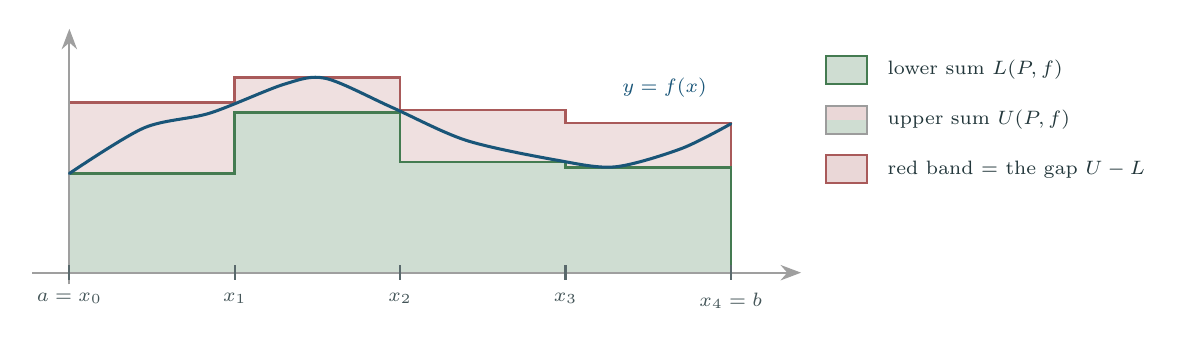
\begin{tikzpicture}[scale=1.05]
    % --- filled bands first; axes and curve go on top ---
    % upper rectangles (light red)
    \fill[thmcolor!14] (0,0) rectangle (2,2.06);
    \fill[thmcolor!14] (2,0) rectangle (4,2.36);
    \fill[thmcolor!14] (4,0) rectangle (6,1.97);
    \fill[thmcolor!14] (6,0) rectangle (8,1.81);
    % lower rectangles (light green, on top of the red)
    \fill[proofcolor!22] (0,0) rectangle (2,1.2);
    \fill[proofcolor!22] (2,0) rectangle (4,1.94);
    \fill[proofcolor!22] (4,0) rectangle (6,1.34);
    \fill[proofcolor!22] (6,0) rectangle (8,1.27);
    % staircase outlines (soft)
    \draw[thmcolor!75, line width=0.9pt]
      (0,2.06) -| (2,2.36) -| (4,1.97) -| (6,1.81) -| (8,0);
    \draw[proofcolor!85, line width=0.9pt]
      (0,1.2) -| (2,1.94) -| (4,1.34) -| (6,1.27) -| (8,0);
    % --- axes on top of the bands ---
    \draw[axisln] (-0.45,0) -- (8.85,0);
    \draw[axisln] (0,-0.14) -- (0,2.95);
    % partition ticks and labels
    \foreach \x/\lab in {0/{a=x_0}, 2/{x_1}, 4/{x_2}, 6/{x_3}, 8/{x_4=b}} {
      \draw[mDarkTeal!75, line width=0.8pt] (\x,0.09) -- (\x,-0.09);
      \node[mDarkTeal!85, font=\scriptsize, below=1pt] at (\x,-0.09) {$\lab$};
    }
    % --- curve last ---
    \draw[curveln, line width=1.1pt, defcolor] plot[smooth] coordinates
      {(0,1.2) (0.9,1.75) (1.7,1.93) (2.6,2.28) (3.1,2.35) (3.9,2.0)
       (4.8,1.6) (5.9,1.36) (6.6,1.28) (7.4,1.5) (8,1.8)};
    \node[defcolor, font=\scriptsize, above] at (7.2,2.0) {$y = f(x)$};
    % --- legend with swatches ---
    \fill[proofcolor!22] (9.15,2.28) rectangle +(0.5,0.34);
    \draw[proofcolor!85, line width=0.7pt] (9.15,2.28) rectangle +(0.5,0.34);
    \node[mDarkTeal, font=\scriptsize, anchor=west] at (9.78,2.45)
      {lower sum $L(P,f)$};
    \fill[proofcolor!22] (9.15,1.68) rectangle +(0.5,0.17);
    \fill[thmcolor!18] (9.15,1.85) rectangle +(0.5,0.17);
    \draw[remcolor!60, line width=0.7pt] (9.15,1.68) rectangle +(0.5,0.34);
    \node[mDarkTeal, font=\scriptsize, anchor=west] at (9.78,1.85)
      {upper sum $U(P,f)$};
    \fill[thmcolor!18] (9.15,1.08) rectangle +(0.5,0.34);
    \draw[thmcolor!75, line width=0.7pt] (9.15,1.08) rectangle +(0.5,0.34);
    \node[mDarkTeal, font=\scriptsize, anchor=west] at (9.78,1.25)
      {red band $=$ the \alert{gap} $U - L$};
  \end{tikzpicture}
  \end{center}

  \note{
    This picture is the whole section in one image. The blue curve is
    the graph of a bounded function "f" on the interval from "a" to
    "b". We chop the interval into pieces using the partition points
    "x" sub 0 through "x" sub 4 on the horizontal axis. Over each piece
    we build two rectangles: a green one whose height is the infimum of
    "f" on that piece, and a taller one reaching up to the supremum of
    "f" on that piece. The green area is the lower sum: it
    underestimates the area under the curve. The green and red together
    form the upper sum, an overestimate. The true area, whatever it
    is, is trapped between them, and the visible red band is exactly
    the gap between the two estimates; the legend on the right records
    this color code. Integrability will mean: by
    choosing the partition cleverly, the red band can be made as thin
    as we please. Now let's turn the picture into definitions.
  }
\end{frame}

}

{
\usebackgroundtemplate{%
  
\includegraphics[width=\paperwidth,height=\paperheight,keepaspectratio=false]{chapter_06_bg_02.png}%
}
\section{The Riemann Integral}

\begin{frame}{Definition 6.1: Partitions}
  \begin{defblock}{Definition 6.1 (partition)}
    A \alert{partition} $P$ of $[a,b]$ is a finite set of points
    $x_0, x_1, \dots, x_n$ with
    \[
      a = x_0 \leq x_1 \leq \cdots \leq x_{n-1} \leq x_n = b.
    \]
    We write $\ \Delta x_i = x_i - x_{i-1}$ \quad $(i = 1, \dots, n)$.
  \end{defblock}

  \vspace{0.3em}
  \begin{center}
  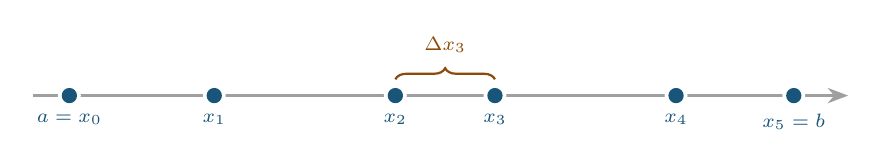
\begin{tikzpicture}[scale=1.15]
    \draw[axisln] (-0.4,0) -- (8.6,0);
    \foreach \x/\lab in {0/{a=x_0}, 1.6/{x_1}, 3.6/{x_2}, 4.7/{x_3}, 6.7/{x_4}, 8/{x_5=b}} {
      \dotpt{defcolor}{(\x,0)}
      \node[defcolor, font=\scriptsize, below=3pt] at (\x,0) {$\lab$};
    }
    \draw[decorate,decoration={brace,amplitude=4pt},thick,excolor]
      (3.6,0.18) -- (4.7,0.18);
    \node[excolor, font=\scriptsize, above=6pt] at (4.15,0.18) {$\Delta x_3$};
  \end{tikzpicture}
  \end{center}

  \note{
    We start with Definition 6.1. A partition of the interval from "a"
    to "b" is just a finite set of division points, listed on the
    slide: the first point is "a", the last point is "b", and the
    points increase, or at least never decrease, in between. On the
    number line you see a partition with six points, "x" sub 0 through
    "x" sub 5. The symbol delta "x" sub "i" denotes the length of
    subinterval number "i", the distance from "x" sub "i" minus 1 to
    "x" sub "i"; the orange brace marks one of them, delta "x" sub 3. Notice that the
    subintervals may have completely different lengths; nothing forces
    the partition to be uniform. Next we use a partition to build the
    two sums from our opening picture.
  }
\end{frame}

% --- Build 1/2 ---
\begin{frame}{Definition 6.1: Upper and Lower Sums}
  \hl{Let $f$ be \alert{bounded} on $[a,b]$. For a partition $P$, put}
  \begin{defblock}{Sup and inf on each subinterval}
    $M_i = \sup f(x) \quad (x_{i-1} \leq x \leq x_i), \qquad
     m_i = \inf f(x) \quad (x_{i-1} \leq x \leq x_i).$
  \end{defblock}

  \note{
    Now let "f" be a bounded real function on the interval; boundedness
    is essential and will stay in force for the whole chapter. Given a
    partition, we look at "f" on each subinterval separately. On
    subinterval number "i", capital "M" sub "i" is the supremum of the
    values of "f", and lowercase "m" sub "i" is their infimum. Both
    exist as finite numbers precisely because "f" is bounded; this is
    the least upper bound property of the real numbers doing its job.
    These are the heights of the red and green rectangles from our
    picture. From them we now build the two sums.
  }
\end{frame}

% --- Build 2/2 ---
\begin{frame}{Definition 6.1: Upper and Lower Sums}
  \hl{Let $f$ be \alert{bounded} on $[a,b]$. For a partition $P$, put}
  \begin{defblock}{Sup and inf on each subinterval}
    $M_i = \sup f(x) \quad (x_{i-1} \leq x \leq x_i), \qquad
     m_i = \inf f(x) \quad (x_{i-1} \leq x \leq x_i).$
  \end{defblock}

  \begin{defblock}{Upper and lower sums}
    \[
      U(P,f) = \sum_{i=1}^{n} M_i\,\Delta x_i, \qquad
      L(P,f) = \sum_{i=1}^{n} m_i\,\Delta x_i.
    \]
  \end{defblock}

  \vspace{0.2em}
  \hl{Always $L(P,f) \leq U(P,f)$, since $m_i \leq M_i$.}

  \note{
    The upper sum, capital "U" of "P" and "f", adds up supremum times
    length over all subintervals: each term "M" sub "i" times delta "x" sub
    "i" is the area of one tall rectangle. The lower sum, capital "L"
    of "P" and "f", does the same with the infima, giving the total
    green area. Since on every subinterval the infimum is at most the
    supremum, the lower sum never exceeds the upper sum for the same
    partition. Every reasonable notion of area under the graph must
    land between these two numbers. That observation motivates the next
    definition.
  }
\end{frame}

% --- Build 1/2 ---
\begin{frame}{Definition 6.1: Upper and Lower Integrals}
  \begin{defblock}{Upper and lower Riemann integrals}
    \[
      \overline{\int_a^b} f\,dx = \inf_P\, U(P,f), \ \ \text{(1)}
      \qquad
      \underline{\int_a^b} f\,dx = \sup_P\, L(P,f), \ \ \text{(2)}
    \]
    the inf and sup taken over \alert{all} partitions $P$ of $[a,b]$.
  \end{defblock}

  \note{
    To get rid of the dependence on the particular partition, we now
    optimize over all of them. Equation 1 defines the upper Riemann
    integral of "f": the infimum of all upper sums, the best possible
    overestimate. Equation 2 defines the lower Riemann integral: the
    supremum of all lower sums, the best possible underestimate. Note
    the direction of each optimization: upper sums are pushed down,
    lower sums are pushed up, and the two bars over and under the
    integral signs record which is which. The obvious question is
    whether the two sides meet.
  }
\end{frame}

% --- Build 2/2 ---
\begin{frame}{Definition 6.1: Upper and Lower Integrals}
  \begin{defblock}{Upper and lower Riemann integrals}
    \[
      \overline{\int_a^b} f\,dx = \inf_P\, U(P,f), \ \ \text{(1)}
      \qquad
      \underline{\int_a^b} f\,dx = \sup_P\, L(P,f), \ \ \text{(2)}
    \]
    the inf and sup taken over \alert{all} partitions $P$ of $[a,b]$.
  \end{defblock}

  \begin{defblock}{The Riemann integral}
    If (1) $=$ (2), we say $f$ is \alert{Riemann-integrable}, write
    $f \in \mathscr{R}$, and denote the common value by
    \[
      \int_a^b f\,dx, \ \ \text{(3)} \qquad \text{or} \qquad
      \int_a^b f(x)\,dx. \ \ \text{(4)}
    \]
  \end{defblock}

  \note{
    If the upper and lower integrals are equal, we say that "f" is
    Riemann-integrable on the interval, and we write "f" belongs to
    script "R", where script "R" denotes the class of all
    Riemann-integrable functions. The common value of equations 1 and 2
    is then called the Riemann integral of "f", written as in equation
    3, or, with the variable displayed, as in equation 4. So the
    integral is not defined as a limit of Riemann sums; it is defined
    as the meeting point of an infimum and a supremum. Before asking
    when they meet, let's check that both quantities always make sense.
  }
\end{frame}

\begin{frame}{Upper and Lower Integrals Always Exist}
  \begin{hlbox}
  Since $f$ is bounded, there are numbers $m$, $M$ with
  $m \leq f(x) \leq M$ on $[a,b]$. Hence for \alert{every} $P$:
  \[
    m(b-a) \;\leq\; L(P,f) \;\leq\; U(P,f) \;\leq\; M(b-a).
  \]
  \end{hlbox}

  \begin{remblock}{Consequence}
    The numbers $L(P,f)$, $U(P,f)$ form a \alert{bounded set}: the upper
    and lower integrals are \alert{defined for every bounded $f$}.
    Their \emph{equality} --- integrability --- is the delicate question.
  \end{remblock}

  \note{
    Here is the promised sanity check. Because "f" is bounded, its
    values lie between two fixed numbers, lowercase "m" and capital
    "M". On any subinterval the infimum of "f" is then at least "m"
    and the supremum is at most capital "M", so the displayed chain of
    inequalities holds for every partition: every lower sum is at least
    "m" times the length of the interval, and every upper sum is at
    most capital "M" times that length. The sums therefore form a
    bounded set of real numbers, and the infimum in equation 1 and the
    supremum in equation 2 both exist. As the gray box says, the upper
    and lower integrals are defined for every bounded function, without
    exception. Whether they are equal is the delicate question. To see
    how badly equality can fail, think of the function on the unit
    interval that equals 1 at every rational and 0 at every irrational:
    every subinterval contains points of both kinds, so every upper sum
    is 1 and every lower sum is 0, no matter the partition. Instead of
    studying the question just for the Riemann integral, Rudin
    immediately moves to a more general setting.
  }
\end{frame}

}

{
\usebackgroundtemplate{%
  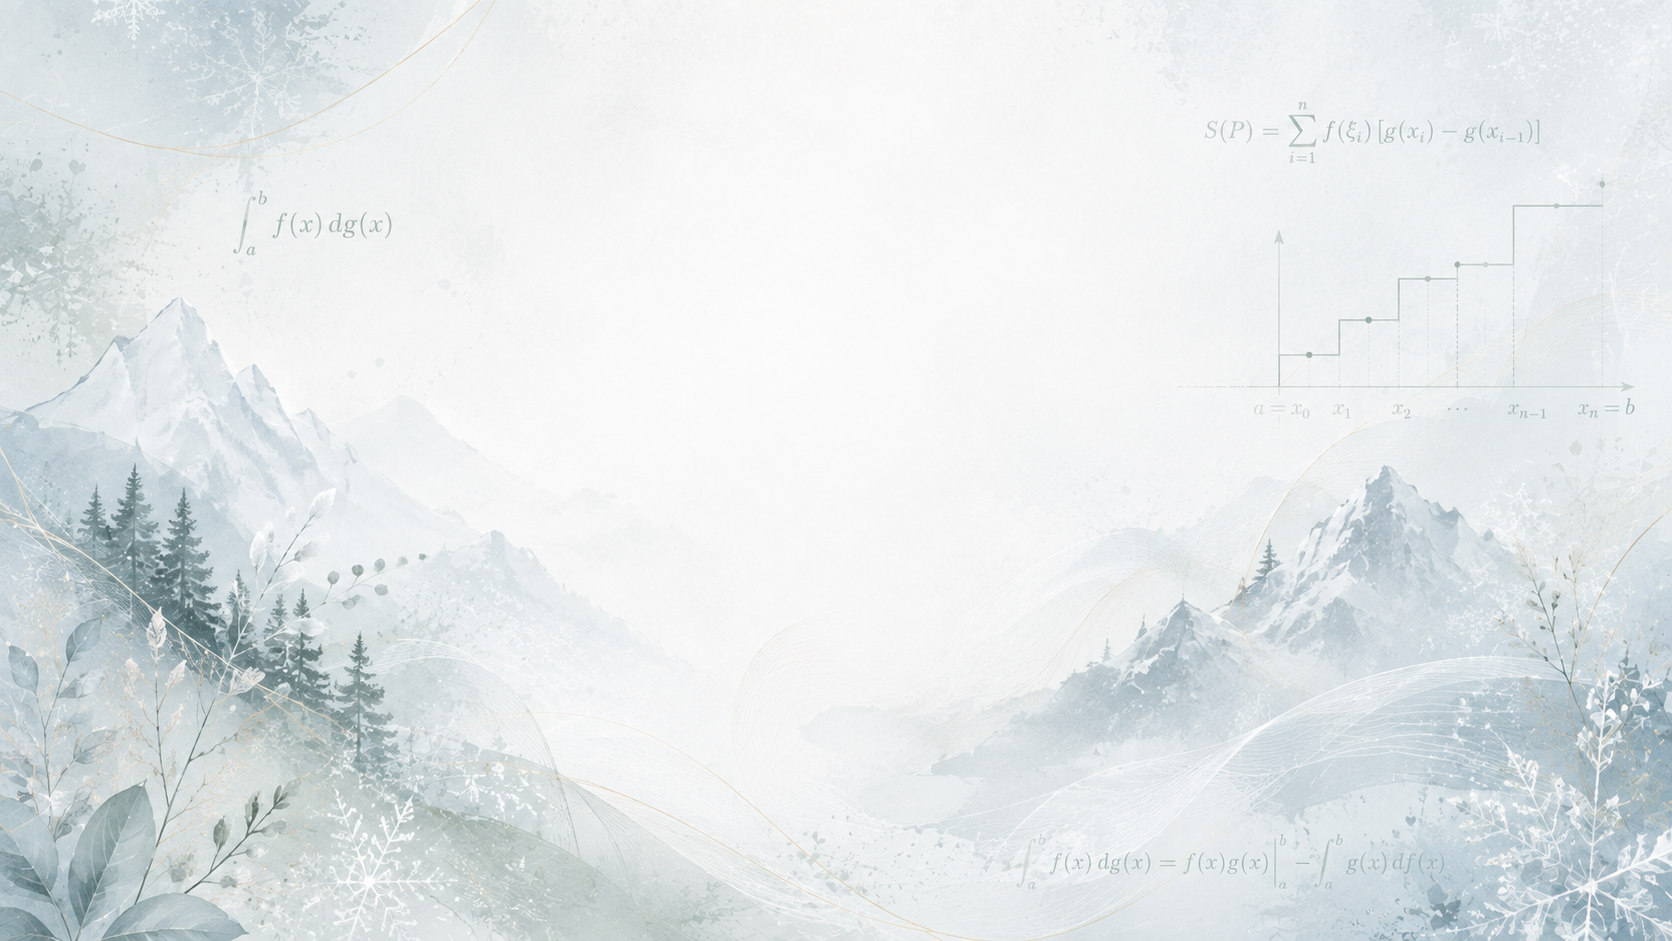
\includegraphics[width=\paperwidth,height=\paperheight,keepaspectratio=false]{chapter_06_bg_03.png}%
}
\section{The Riemann--Stieltjes Integral}

% --- Build 1/2 ---
\begin{frame}{Definition 6.2: An Increasing Weight $\alpha$}
  \begin{defblock}{Definition 6.2 (setup)}
    Let $\alpha$ be \alert{monotonically increasing} on $[a,b]$.
    Since $\alpha(a)$, $\alpha(b)$ are finite, $\alpha$ is bounded.
    For each partition $P$ write
    \[
      \Delta\alpha_i = \alpha(x_i) - \alpha(x_{i-1}) \;\geq\; 0.
    \]
  \end{defblock}

  \begin{center}
  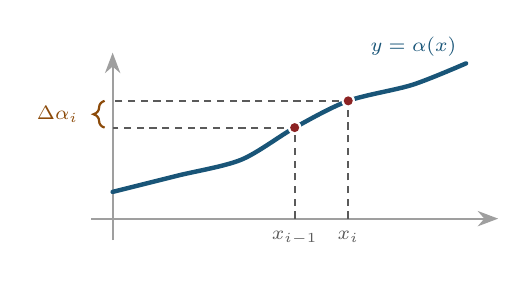
\begin{tikzpicture}[scale=0.68]
    \draw[axisln] (-0.4,0) -- (7.2,0);
    \draw[axisln] (0,-0.4) -- (0,3.1);
    \draw[curveln, defcolor] plot[smooth] coordinates
      {(0,0.5) (1.2,0.8) (2.4,1.1) (3.4,1.7) (4.4,2.2) (5.6,2.5) (6.6,2.9)};
    \node[defcolor, font=\scriptsize, above left] at (6.6,2.85) {$y=\alpha(x)$};
    % projections
    \draw[projln, remcolor] (3.4,0) -- (3.4,1.7) -- (0,1.7);
    \draw[projln, remcolor] (4.4,0) -- (4.4,2.2) -- (0,2.2);
    \dotpt{thmcolor}{(3.4,1.7)}
    \dotpt{thmcolor}{(4.4,2.2)}
    \node[remcolor, font=\scriptsize, below] at (3.4,-0.05) {$x_{i-1}$};
    \node[remcolor, font=\scriptsize, below] at (4.4,-0.05) {$x_i$};
    \draw[decorate,decoration={brace,amplitude=4pt},thick,excolor]
      (-0.15,1.7) -- (-0.15,2.2);
    \node[excolor, font=\scriptsize, left=6pt] at (-0.15,1.95) {$\Delta\alpha_i$};
  \end{tikzpicture}
  \end{center}

  \note{
    Here is the generalization, Definition 6.2. We bring in a second
    function, alpha, which is monotonically increasing on the interval.
    Since its values at "a" and at "b" are finite, alpha is
    automatically bounded. Given a partition, delta alpha sub "i"
    denotes the increase of alpha across subinterval number "i"; since
    alpha is increasing, these numbers are never negative. The diagram
    shows the idea: the blue curve is the graph of alpha, the two
    dashed lines project the subinterval endpoints "x" sub "i" minus 1
    and "x" sub "i" up to the graph and across to the vertical axis,
    and the orange brace marks delta alpha sub "i", the rise of alpha.
    Where the Riemann integral measured a subinterval by its length,
    we now measure it by how much alpha grows across it. Everything
    else is copied word for word, as we see next.
  }
\end{frame}

% --- Build 2/2 ---
\begin{frame}{Definition 6.2: Weighted Sums and Integrals}
  \begin{defblock}{Weighted upper and lower sums}
    For any real $f$ bounded on $[a,b]$ (with $M_i$, $m_i$ as in Def.\ 6.1):
    \[
      U(P,f,\alpha) = \sum_{i=1}^{n} M_i\,\Delta\alpha_i, \qquad
      L(P,f,\alpha) = \sum_{i=1}^{n} m_i\,\Delta\alpha_i,
    \]
    \begin{equation}
      \overline{\int_a^b} f\,d\alpha = \inf_P\, U(P,f,\alpha), \tag{5}
    \end{equation}
    \begin{equation}
      \underline{\int_a^b} f\,d\alpha = \sup_P\, L(P,f,\alpha). \tag{6}
    \end{equation}
  \end{defblock}

  \note{
    Now replace length by the growth of alpha everywhere. The upper sum
    "U" of "P", "f", alpha adds supremum times delta alpha sub "i"
    over the subintervals; the lower sum uses the infima, with capital "M" sub
    "i" and lowercase "m" sub "i" exactly as in Definition 6.1.
    Equations 5 and 6 then define the upper and lower integrals of "f"
    with respect to alpha: the infimum of the upper sums and the
    supremum of the lower sums, over all partitions, just as before.
    The whole structure of Definition 6.1 carries over with delta "x"
    replaced by delta alpha. One more step gives the integral itself.
  }
\end{frame}

\begin{frame}{The Riemann--Stieltjes Integral}
  \begin{defblock}{The integral of $f$ with respect to $\alpha$}
    If (5) $=$ (6), we denote the common value by
    \begin{equation}
      \int_a^b f\,d\alpha \tag{7}
    \end{equation}
    or
    \begin{equation}
      \int_a^b f(x)\,d\alpha(x). \tag{8}
    \end{equation}
    This is the \alert{Riemann--Stieltjes integral} of $f$ with respect
    to $\alpha$ over $[a,b]$; we say $f$ is integrable with respect to
    $\alpha$ and write $f \in \mathscr{R}(\alpha)$.
  \end{defblock}

  \note{
    If the upper and lower integrals with respect to alpha agree, their
    common value is written as in equation 7, or with the variable
    displayed as in equation 8. This number is the Riemann-Stieltjes
    integral, or simply the Stieltjes integral, of "f" with respect to
    alpha over the interval. When it exists we say "f" is integrable
    with respect to alpha in the Riemann sense, and we write "f"
    belongs to script "R" of alpha. So for each increasing weight
    alpha we get a whole class of integrable functions, and the
    membership question depends on both "f" and alpha. Two remarks
    before we move on.
  }
\end{frame}

\begin{frame}{Two Remarks on the Definition}
  \begin{remblock}{The Riemann integral is a special case}
    Taking $\alpha(x) = x$ gives $\Delta\alpha_i = \Delta x_i$:
    Riemann integral is the case $\alpha(x) = x$ of the
    Riemann--Stieltjes integral.
  \end{remblock}

  \vspace{0.4em}
  \begin{remblock}{$\alpha$ can be wild}
    In general, $\alpha$ \alert{need not even be continuous} ---
    step functions are allowed (and will be important!).
  \end{remblock}

  \note{
    First, the ordinary Riemann integral really is a special case: take
    alpha of "x" equal to "x". Then the growth of alpha across a
    subinterval is just its length, delta alpha sub "i" equals delta
    "x" sub "i", and Definition 6.2 collapses to Definition 6.1. So
    everything we prove about the Stieltjes integral automatically
    holds for the ordinary integral. Second, and this is worth
    emphasizing, the weight alpha need not be continuous. Jump
    functions, staircases, are perfectly legal weights, and later in
    the chapter they will let the Stieltjes integral swallow infinite
    series as a special case. That flexibility is the whole point of
    the generalization. Next, a short remark about notation.
  }
\end{frame}

\begin{frame}{The Variable of Integration Is a Dummy}
  \begin{remblock}{Notation}
    We prefer (7) to (8): the letter $x$ in (8) \alert{adds nothing}.
    For instance, (8) is the same as
    \[
      \int_a^b f(y)\,d\alpha(y).
    \]
    The integral depends on $f$, $\alpha$, $a$, $b$ --- \emph{not} on the
    variable of integration. It is analogous to the index of summation:
    \[
      \sum_{i=1}^{n} c_i \qquad \text{and} \qquad \sum_{k=1}^{n} c_k
      \qquad \text{both mean} \qquad c_1 + c_2 + \cdots + c_n.
    \]
  \end{remblock}

  \note{
    A few words about notation. Rudin prefers the bare form of
    equation 7, without the letter "x", because the variable of
    integration is a dummy: it can be renamed at will. Writing the
    integral of "f" of "y" "d" alpha of "y" means exactly the same
    thing. The integral is a number determined by four pieces of data:
    the function "f", the weight alpha, and the endpoints "a" and "b".
    The slide shows the perfect analogy: a finite sum does not depend
    on whether its index is called "i" or "k"; both symbols denote "c"
    sub 1 plus "c" sub 2 up to "c" sub "n". Of course, no harm is done
    by inserting the variable, and sometimes it is convenient. Now we
    set our standing conventions and begin investigating existence.
  }
\end{frame}

\begin{frame}{Standing Assumptions}
  \begin{remblock}{For the rest of this chapter (unless said otherwise)}
    \begin{itemize}
      \item $f$ is \alert{real and bounded} on $[a,b]$
      \item $\alpha$ is \alert{monotonically increasing} on $[a,b]$
      \item When no confusion can arise, we write $\displaystyle\int$
        for $\displaystyle\int_a^b$
    \end{itemize}
  \end{remblock}

  \vspace{0.4em}
  \hl{\textbf{Goal:} decide \alert{when} $f \in \mathscr{R}(\alpha)$.}

  \note{
    Before diving into theorems, we fix the standing assumptions, so
    that they do not have to be repeated in every statement. From now
    on, "f" is a real bounded function on the interval, and alpha is
    monotonically increasing on it. And when no misunderstanding is
    possible, the integral sign is written without its limits. The
    goal for the rest of this episode is on the slide: to decide when
    "f" belongs to script "R" of alpha, that is, when the upper and
    lower integrals meet. The key tool is the idea of refining a
    partition, which we develop now.
  }
\end{frame}

}

{
\usebackgroundtemplate{%
  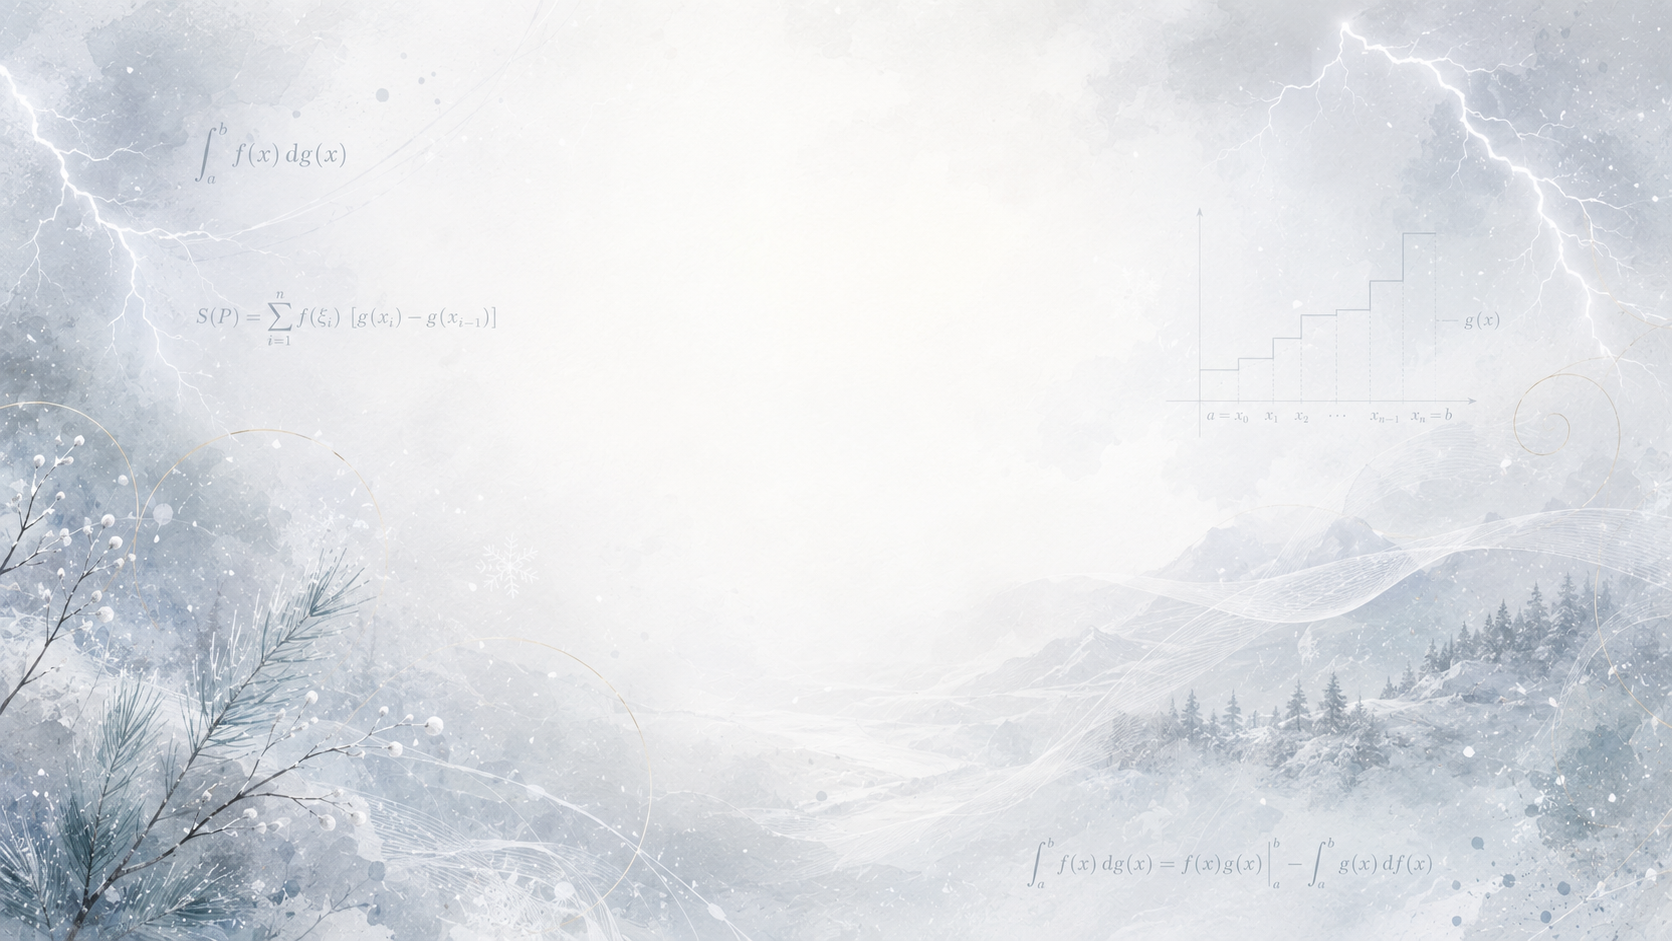
\includegraphics[width=\paperwidth,height=\paperheight,keepaspectratio=false]{chapter_06_bg_04.png}%
}
\section{Refinements}

\begin{frame}{Definition 6.3: Refinements}
  \begin{defblock}{Definition 6.3}
    $P^*$ is a \alert{refinement} of $P$ if $P^* \supset P$
    (every point of $P$ is a point of $P^*$).
    Given $P_1$, $P_2$, their \alert{common refinement} is
    $P^* = P_1 \cup P_2$.
  \end{defblock}

  \vspace{0.3em}
  \begin{center}
  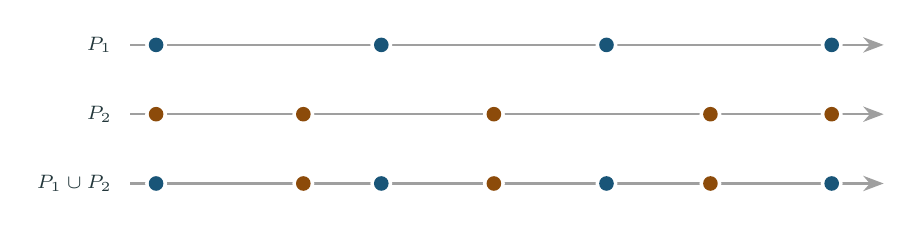
\begin{tikzpicture}[scale=1.1]
    % P1
    \draw[axisln] (-0.3,1.6) -- (8.4,1.6);
    \node[font=\scriptsize, mDarkTeal, left] at (-0.4,1.6) {$P_1$};
    \foreach \x in {0, 2.6, 5.2, 7.8} { \dotpt{defcolor}{(\x,1.6)} }
    % P2
    \draw[axisln] (-0.3,0.8) -- (8.4,0.8);
    \node[font=\scriptsize, mDarkTeal, left] at (-0.4,0.8) {$P_2$};
    \foreach \x in {0, 1.7, 3.9, 6.4, 7.8} { \dotpt{excolor}{(\x,0.8)} }
    % common refinement
    \draw[axisln] (-0.3,0) -- (8.4,0);
    \node[font=\scriptsize, mDarkTeal, left] at (-0.4,0) {$P_1 \cup P_2$};
    \foreach \x in {0, 2.6, 5.2, 7.8} { \dotpt{defcolor}{(\x,0)} }
    \foreach \x in {1.7, 3.9, 6.4} { \dotpt{excolor}{(\x,0)} }
  \end{tikzpicture}
  \end{center}

  \note{
    Definition 6.3 introduces the key technical device of the section.
    A partition "P" star is a refinement of "P" if it contains every
    point of "P", and possibly more; we only add division points,
    never remove them. Given two partitions "P" sub 1 and "P" sub 2,
    their common refinement is simply their union, the partition
    containing the points of both. The diagram shows all three number
    lines: on top, "P" sub 1 with its blue points; in the middle, "P"
    sub 2 with its orange points; and at the bottom their union, where
    both families of points appear together. The common refinement is
    the coarsest partition that refines both. Why refine? Because
    refining always improves both of our estimates, as the next
    theorem shows.
  }
\end{frame}

\begin{frame}{Theorem 6.4: Refining Improves Both Sums}
  \begin{thmblock}{Theorem 6.4}
    If $P^*$ is a refinement of $P$, then
    \begin{equation}
      L(P,f,\alpha) \leq L(P^*,f,\alpha) \tag{9}
    \end{equation}
    and
    \begin{equation}
      U(P^*,f,\alpha) \leq U(P,f,\alpha). \tag{10}
    \end{equation}
  \end{thmblock}

  \vspace{0.3em}
  \begin{hlbox}
  \textbf{Key idea:} adding points can only \alert{tighten} the trap:
  lower sums go up, upper sums come down.
  \end{hlbox}

  \note{
    Theorem 6.4 says that refining a partition never hurts. Inequality
    9: the lower sum computed with the finer partition "P" star is at
    least the lower sum for "P"; refining pushes lower sums up.
    Inequality 10: the upper sum for "P" star is at most the upper sum
    for "P"; refining pulls upper sums down. Together, the trap around
    the would-be integral only tightens as we add division points.
    Intuitively, more points mean the rectangles can hug the graph
    more closely from both sides. The proof is a pleasant computation,
    and it is enough to understand what happens when we add a single
    point.
  }
\end{frame}

\begin{frame}{Proof of Theorem 6.4 --- Step 1: One Extra Point}
  \begin{proofblock}{Step 1: Setup}
    Suppose first $P^*$ has \alert{just one more point} $x^*$ than $P$,
    with $x_{i-1} < x^* < x_i$. Put
    \[
      w_1 = \inf f(x) \quad (x_{i-1} \leq x \leq x^*), \qquad
      w_2 = \inf f(x) \quad (x^* \leq x \leq x_i).
    \]
    Then $\ w_1 \geq m_i$ and $w_2 \geq m_i$, where
    $m_i = \inf f(x)$ on $[x_{i-1}, x_i]$.
  \end{proofblock}

  \vspace{0.3em}
  \hl{\textbf{Why:} an inf over a \alert{smaller} set can only be
  \alert{larger}.}

  \note{
    To prove inequality 9, suppose first that "P" star contains just
    one extra point, call it "x" star, and say it falls strictly
    between the consecutive points "x" sub "i" minus 1 and "x" sub "i"
    of "P". The old subinterval splits into two halves. Let "w" sub 1
    be the infimum of "f" on the left half, and "w" sub 2 the infimum
    on the right half. The key observation is at the bottom of the
    block: both "w" sub 1 and "w" sub 2 are at least "m" sub "i", the
    infimum over the whole subinterval. The reason is stated below the
    box: shrinking the set over which we take an infimum can only
    raise the infimum, because there are fewer candidates competing to
    be small. Let's see this in a picture before computing.
  }
\end{frame}

\begin{frame}[c]{The Picture: Why Lower Sums Rise}
  \begin{center}
  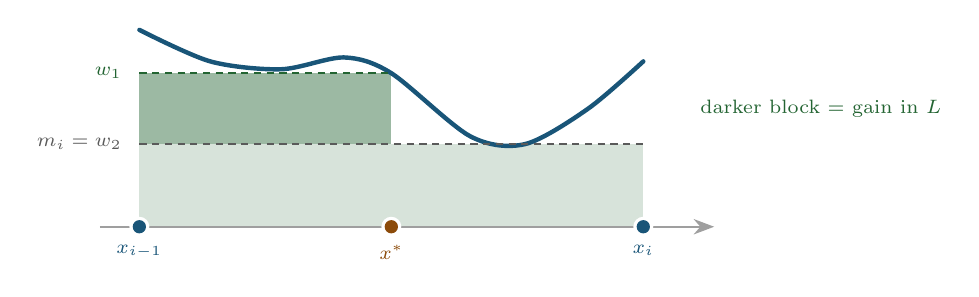
\begin{tikzpicture}[scale=1.0]
    % baseline rectangle at height m_i over whole interval
    \fill[proofcolor!18] (0,0) rectangle (6.4,1.05);
    % improved left rectangle at w1
    \fill[proofcolor!45] (0,1.05) rectangle (3.2,1.95);
    % axis
    \draw[axisln] (-0.5,0) -- (7.3,0);
    % curve: decreasing then min in right half then up
    \draw[curveln, defcolor] plot[smooth] coordinates
      {(0,2.5) (0.9,2.1) (1.8,2.0) (2.6,2.15) (3.2,1.95) (4.2,1.15)
       (4.9,1.05) (5.7,1.5) (6.4,2.1)};
    % levels
    \draw[projln, proofcolor] (0,1.95) -- (3.2,1.95);
    \node[proofcolor, font=\scriptsize, left] at (-0.1,1.95) {$w_1$};
    \draw[projln, remcolor] (0,1.05) -- (6.4,1.05);
    \node[remcolor, font=\scriptsize, left] at (-0.1,1.05) {$m_i = w_2$};
    % partition points
    \foreach \x/\lab in {0/{x_{i-1}}, 6.4/{x_i}} {
      \dotpt{defcolor}{(\x,0)}
      \node[defcolor, font=\scriptsize, below=3pt] at (\x,0) {$\lab$};
    }
    \dotpt{excolor}{(3.2,0)}
    \node[excolor, font=\scriptsize, below=3pt] at (3.2,0) {$x^*$};
    % gain label
    \node[proofcolor, font=\scriptsize, anchor=west] at (7.0,1.5)
      {darker block $=$ \alert{gain} in $L$};
  \end{tikzpicture}
  \end{center}

  \note{
    Here is the geometry. The blue curve is "f" on the subinterval
    from "x" sub "i" minus 1 to "x" sub "i", and the orange point "x"
    star is the new division point in the middle. Before refining, the
    lower sum used one flat rectangle over the whole subinterval, at
    the height "m" sub "i", the overall infimum; that is the light
    green slab. In this picture "f" dips lowest in the right half, so
    the right infimum "w" sub 2 coincides with "m" sub "i". But on the
    left half the function stays high, so the left infimum "w" sub 1
    is strictly larger, and the lower rectangle over the left half can
    rise to that level. The darker green block is precisely the area
    gained by the lower sum when the point "x" star is added. The
    upper sums behave symmetrically: refinement lets the tall
    rectangles come down. Now we compute the gain exactly.
  }
\end{frame}

\begin{frame}{Proof of Theorem 6.4 --- Step 2: Compute the Gain}
  \begin{proofblock}{Step 2: The gain is nonnegative}
    \small
    \begin{align*}
      L(P^*,f,\alpha) - L(P,f,\alpha)
      &= w_1[\alpha(x^*) - \alpha(x_{i-1})]
        + w_2[\alpha(x_i) - \alpha(x^*)] \\
      &\qquad - m_i[\alpha(x_i) - \alpha(x_{i-1})] \\
      &= (w_1 - m_i)[\alpha(x^*) - \alpha(x_{i-1})] \\
      &\qquad + (w_2 - m_i)[\alpha(x_i) - \alpha(x^*)] \;\geq\; 0.
    \end{align*}
  \end{proofblock}

  \vspace{0.3em}
  \hl{Each factor is $\geq 0$: \ $w_1, w_2 \geq m_i$ \ and \ $\alpha$ is
  \alert{increasing}.}

  \note{
    Now the computation. All terms of the two lower sums agree except
    those coming from the split subinterval, so the difference of the
    lower sums is exactly what is displayed: the left half contributes
    "w" sub 1 times the rise of alpha over the left half, the right
    half contributes "w" sub 2 times the rise over the right half, and
    we subtract the old term, "m" sub "i" times the rise over the
    whole subinterval. In the second line, the old term is split
    across the two halves and the difference is regrouped into two
    products. Each product is nonnegative: the first factors are
    nonnegative because "w" sub 1 and "w" sub 2 are at least "m" sub
    "i", and the second factors are nonnegative because alpha is
    increasing. So the gain is at least zero, which is inequality 9
    for one extra point.
  }
\end{frame}

\begin{frame}{Proof of Theorem 6.4 --- Step 3: Iterate}
  \begin{proofblock}{Step 3: Finish}
    If $P^*$ contains $k$ points more than $P$, repeat the argument
    $k$ times: this proves (9). The proof of (10) is
    \alert{analogous} (with sups in place of infs). \qed
  \end{proofblock}

  \vspace{0.4em}
  \hl{\textbf{Technique:} reduce to the \alert{one-point} case, then iterate.}

  \note{
    The general case follows by iteration. If the refinement "P" star
    has "k" extra points, insert them one at a time: each insertion is
    the situation we just analyzed, so each insertion can only
    increase the lower sum, and after "k" steps inequality 9 is
    proved. The companion inequality 10, for upper sums, is proved the
    same way, with suprema in place of infima; there, splitting a
    subinterval can only lower the suprema on the two halves, so the
    upper sum comes down. The technique is worth noting: reduce to
    the smallest possible change, one added point, then iterate. With
    Theorem 6.4 in hand, we can compare the lower and upper integrals
    themselves.
  }
\end{frame}

\begin{frame}{Theorem 6.5: Lower Never Exceeds Upper}
  \begin{thmblock}{Theorem 6.5}
    \[
      \underline{\int_a^b} f\,d\alpha \;\leq\; \overline{\int_a^b} f\,d\alpha.
    \]
  \end{thmblock}

  \vspace{0.3em}
  \begin{hlbox}
  Not obvious! \ (2) and (5) involve \alert{different} partitions:
  we must compare $L(P_1, f, \alpha)$ with $U(P_2, f, \alpha)$ for
  \alert{arbitrary} $P_1$, $P_2$.
  \end{hlbox}

  \note{
    Theorem 6.5 states what the notation has been suggesting all
    along: the lower integral is at most the upper integral. Let me
    stress that this is not automatic. For a single partition we know
    the lower sum is at most the upper sum. But the lower integral is
    a supremum over all partitions, and the upper integral is an
    infimum over all partitions, so we must compare the lower sum for
    one partition with the upper sum for a completely different one.
    The common refinement is exactly the bridge between two unrelated
    partitions, and the proof is a one-line chain of inequalities.
    Let's see it.
  }
\end{frame}

\begin{frame}{Proof of Theorem 6.5 --- The Chain}
  \begin{proofblock}{Proof}
    \small
    Let $P^*$ be the common refinement of $P_1$ and $P_2$. By Theorem 6.4,
    \[
      L(P_1,f,\alpha) \leq L(P^*,f,\alpha) \leq U(P^*,f,\alpha)
      \leq U(P_2,f,\alpha).
    \]
    Hence
    \begin{equation}
      L(P_1,f,\alpha) \leq U(P_2,f,\alpha). \tag{11}
    \end{equation}
    Fix $P_2$, take $\sup$ over all $P_1$:
    \begin{equation}
      \underline{\int} f\,d\alpha \leq U(P_2,f,\alpha). \tag{12}
    \end{equation}
    Take $\inf$ over all $P_2$ in (12): \quad
    $\underline{\int} f\,d\alpha \leq \overline{\int} f\,d\alpha$. \qed
  \end{proofblock}

  \note{
    Given two arbitrary partitions "P" sub 1 and "P" sub 2, let "P"
    star be their common refinement. Now read the chain on the slide.
    The first inequality is Theorem 6.4: refining raises lower sums.
    The middle inequality holds because for the single partition "P"
    star, the lower sum is at most the upper sum. The last is Theorem
    6.4 again: refining lowers upper sums. The ends of the chain give
    inequality 11: every lower sum is at most every upper sum, no
    matter how unrelated the two partitions are. Now optimize. Fixing
    "P" sub 2 and taking the supremum over all "P" sub 1, the left
    side becomes the lower integral; that is inequality 12. Then
    taking the infimum over all "P" sub 2 turns the right side into
    the upper integral, and the theorem is proved. The trap is now
    fully set up, and we can ask when it closes.
  }
\end{frame}

}

{
\usebackgroundtemplate{%
  
\includegraphics[width=\paperwidth,height=\paperheight,keepaspectratio=false]{chapter_06_bg_05.png}%
}
\section{The Cauchy Criterion for Integrability}

\begin{frame}{Theorem 6.6: The Integrability Criterion}
  \begin{thmblock}{Theorem 6.6}
    $f \in \mathscr{R}(\alpha)$ on $[a,b]$ \ \alert{if and only if} \
    for every $\varepsilon > 0$ there exists a partition $P$ such that
    \begin{equation}
      U(P,f,\alpha) - L(P,f,\alpha) < \varepsilon. \tag{13}
    \end{equation}
  \end{thmblock}

  \vspace{0.3em}
  \begin{hlbox}
  \textbf{Key idea:} no need to compute either integral ---
  just make the \alert{red band} thin with \emph{one} good partition.
  \end{hlbox}

  \note{
    Here is the heart of the section, Theorem 6.6. It says "f" is
    integrable with respect to alpha if and only if, for every
    positive epsilon, some partition "P" satisfies inequality 13: its
    upper sum and lower sum differ by less than epsilon. Think of it
    as a Cauchy criterion for integrals: exactly as a Cauchy sequence
    is one whose terms squeeze together without knowing the limit,
    condition 13 certifies integrability without computing either the
    upper or the lower integral. In the language of our opening
    picture, integrability means the red band, the gap between the
    upper and lower rectangles, can be made as thin as we like by a
    single well-chosen partition. Nearly every integrability proof in
    this chapter goes through this criterion. Let's prove both
    directions.
  }
\end{frame}

\begin{frame}{Proof of Theorem 6.6 --- ``If'': The Squeeze}
  \begin{proofblock}{(13) for every $\varepsilon$ $\;\Longrightarrow\;$ $f \in \mathscr{R}(\alpha)$}
    For \alert{every} $P$:
    \[
      L(P,f,\alpha) \;\leq\; \underline{\int} f\,d\alpha
      \;\leq\; \overline{\int} f\,d\alpha \;\leq\; U(P,f,\alpha).
    \]
    Thus (13) implies
    \[
      0 \;\leq\; \overline{\int} f\,d\alpha - \underline{\int} f\,d\alpha
      \;<\; \varepsilon.
    \]
    True for every $\varepsilon > 0$
    $\;\Longrightarrow\;$ the two integrals are \alert{equal}:
    $f \in \mathscr{R}(\alpha)$.
  \end{proofblock}

  \note{
    First suppose condition 13 can be satisfied for every epsilon. The
    chain at the top holds for any partition whatsoever: the lower sum
    is at most the lower integral, since that integral is a supremum
    of lower sums; the lower integral is at most the upper integral by
    Theorem 6.5; and the upper integral, being an infimum of upper
    sums, is at most the upper sum. So both integrals are squeezed
    inside the same interval of length less than epsilon, and their
    difference, which is nonnegative, is less than epsilon. Since
    epsilon was arbitrary, the difference must be zero. The two
    integrals agree, which is exactly the definition of "f" belonging
    to script "R" of alpha. Now the converse.
  }
\end{frame}

\begin{frame}{Proof of Theorem 6.6 --- ``Only If'': Step 1}
  \begin{proofblock}{Step 1: Two good partitions}
    Suppose $f \in \mathscr{R}(\alpha)$, let $\varepsilon > 0$.
    Since $\int f\,d\alpha$ is both $\sup_P L$ and $\inf_P U$, there
    exist partitions $P_1$, $P_2$ with
    \begin{equation}
      U(P_2,f,\alpha) - \int f\,d\alpha < \frac{\varepsilon}{2}, \tag{14}
    \end{equation}
    \begin{equation}
      \int f\,d\alpha - L(P_1,f,\alpha) < \frac{\varepsilon}{2}. \tag{15}
    \end{equation}
  \end{proofblock}

  \vspace{0.3em}
  \hl{\textbf{Problem:} two \alert{different} partitions.
  \quad \textbf{Fix:} their \alert{common refinement}.}

  \note{
    Conversely, suppose "f" is integrable, and let epsilon be given.
    The integral is simultaneously the supremum of all lower sums and
    the infimum of all upper sums. By the approximation property of
    the infimum, some partition "P" sub 2 has its upper sum within
    epsilon over 2 above the integral; that is inequality 14. By the
    approximation property of the supremum, some partition "P" sub 1
    has its lower sum within epsilon over 2 below the integral; that
    is inequality 15. The familiar difficulty appears again: these are
    two different partitions, and condition 13 needs a single one. The
    fix is the one we already know: pass to the common refinement,
    which is at least as good as each of them.
  }
\end{frame}

\begin{frame}{Proof of Theorem 6.6 --- ``Only If'': Step 2}
  \begin{proofblock}{Step 2: Merge and chain}
    Let $P$ be the common refinement of $P_1$ and $P_2$. Theorem 6.4
    with (14) and (15) gives
    \[
      U(P,f,\alpha) \leq U(P_2,f,\alpha)
      < \int f\,d\alpha + \frac{\varepsilon}{2}
      < L(P_1,f,\alpha) + \varepsilon
      \leq L(P,f,\alpha) + \varepsilon,
    \]
    so (13) holds for this $P$. \qed
  \end{proofblock}

  \note{
    Let "P" be the common refinement of "P" sub 1 and "P" sub 2, and
    follow the chain. First, "U" of "P" is at most "U" of "P" sub 2,
    because refining lowers upper sums. Next, by inequality 14, "U" of
    "P" sub 2 is less than the integral plus epsilon over 2. Next, by
    inequality 15, the integral is less than the lower sum of "P" sub
    1 plus epsilon over 2; adding epsilon over 2 to both sides, the
    integral plus epsilon over 2 is less than "L" of "P" sub 1 plus
    epsilon. Finally, "L" of "P" sub 1 is at most "L" of "P", because
    refining raises lower sums. Reading the two ends: the upper sum of
    "P" exceeds its lower sum by less than epsilon, which is condition
    13 for the single partition "P". The criterion is proved, and we
    now record three useful companions.
  }
\end{frame}

% --- Build 1/3 ---
\begin{frame}{Theorem 6.7: Working with the Criterion}
  \begin{thmblock}{Theorem 6.7(a)}
    \small
    If (13) holds for some $P$ and some $\varepsilon$, then (13) holds
    (with the same $\varepsilon$) for \alert{every refinement} of $P$.
  \end{thmblock}

  \note{
    Theorem 6.7 collects three facts that make the criterion practical
    to use. Part "a": once a partition satisfies condition 13, every
    refinement of it satisfies condition 13 with the same epsilon.
    Good partitions stay good when refined, so we are always free to
    add extra points, for instance to include some special point we
    care about, without spoiling the estimate. Next, part "b" tells
    us what condition 13 says about values of "f" sampled inside the
    subintervals.
  }
\end{frame}

% --- Build 2/3 ---
\begin{frame}{Theorem 6.7: Working with the Criterion}
  \begin{thmblock}{Theorem 6.7(a)}
    \small
    If (13) holds for some $P$ and some $\varepsilon$, then (13) holds
    (with the same $\varepsilon$) for \alert{every refinement} of $P$.
  \end{thmblock}

  \begin{thmblock}{Theorem 6.7(b)}
    \small
    If (13) holds for $P = \{x_0, \dots, x_n\}$ and $s_i$, $t_i$ are
    \alert{arbitrary points} in $[x_{i-1}, x_i]$, then
    $\ \sum_{i=1}^{n} |f(s_i) - f(t_i)|\,\Delta\alpha_i < \varepsilon$.
  \end{thmblock}

  \note{
    Part "b": suppose condition 13 holds for a partition, and in each
    subinterval pick two sample points, "s" sub "i" and "t" sub "i",
    completely arbitrarily. Then the sum of the differences of the
    sampled values, in absolute value, weighted by delta alpha sub
    "i", is still less than epsilon. In words: on a good partition,
    "f" cannot oscillate much within the subintervals, on average
    with respect to the weight alpha. Finally, part "c" connects all
    this to the sums one actually computes in practice.
  }
\end{frame}

% --- Build 3/3 ---
\begin{frame}{Theorem 6.7: Working with the Criterion}
  \begin{thmblock}{Theorem 6.7(a)}
    \small
    If (13) holds for some $P$ and some $\varepsilon$, then (13) holds
    (with the same $\varepsilon$) for \alert{every refinement} of $P$.
  \end{thmblock}

  \begin{thmblock}{Theorem 6.7(b)}
    \small
    If (13) holds for $P = \{x_0, \dots, x_n\}$ and $s_i$, $t_i$ are
    \alert{arbitrary points} in $[x_{i-1}, x_i]$, then
    $\ \sum_{i=1}^{n} |f(s_i) - f(t_i)|\,\Delta\alpha_i < \varepsilon$.
  \end{thmblock}

  \begin{thmblock}{Theorem 6.7(c)}
    \small
    If $f \in \mathscr{R}(\alpha)$ and the hypotheses of (b) hold, then
    $\ \bigl|\sum_{i=1}^{n} f(t_i)\,\Delta\alpha_i
    - \int_a^b f\,d\alpha\bigr| < \varepsilon$.
  \end{thmblock}

  \note{
    Part "c": if "f" is integrable and the partition satisfies
    condition 13, then any Riemann-Stieltjes sum, formed by sampling
    "f" at arbitrary points "t" sub "i" and weighting by delta alpha
    sub "i", approximates the integral to within epsilon. This is the
    bridge between our definition through suprema and infima and the
    familiar picture of the integral as a limit of sums of sampled
    values. It
    is also the form in which the criterion gets used for numerical
    approximation. The proofs of all three parts are short; let's go
    through them.
  }
\end{frame}

\begin{frame}{Proof of Theorem 6.7 --- Parts (a) and (b)}
  \begin{proofblock}{(a)}
    Refine $P$: by Theorem 6.4, $U$ does not increase and $L$ does not
    decrease, so $U - L$ does not increase. \quad
    $\Rightarrow$ (13) persists.
  \end{proofblock}

  \vspace{0.3em}
  \begin{proofblock}{(b)}
    Both $f(s_i)$ and $f(t_i)$ lie in $[m_i, M_i]$, so
    $|f(s_i) - f(t_i)| \leq M_i - m_i$. Hence
    \[
      \sum_{i=1}^{n} |f(s_i) - f(t_i)|\,\Delta\alpha_i
      \;\leq\; U(P,f,\alpha) - L(P,f,\alpha) \;<\; \varepsilon.
    \]
  \end{proofblock}

  \note{
    Part "a" is immediate from Theorem 6.4: passing to a refinement,
    the upper sum can only shrink and the lower sum can only grow, so
    their difference can only shrink, and if it was below epsilon it
    stays below epsilon. For part "b", look at one subinterval. Both
    sampled values "f" of "s" sub "i" and "f" of "t" sub "i" lie
    between the infimum "m" sub "i" and the supremum "M" sub "i" of
    "f" there, so their difference is at most "M" sub "i" minus "m"
    sub "i", in absolute value. Multiplying by delta alpha sub "i"
    and summing over "i", the left side is at most the sum of the
    oscillations times the weights, which is exactly "U" minus "L",
    and that is less than epsilon by hypothesis. One part remains.
  }
\end{frame}

\begin{frame}{Proof of Theorem 6.7 --- Part (c)}
  \begin{proofblock}{(c)}
    The obvious inequalities
    \[
      L(P,f,\alpha) \;\leq\; \sum f(t_i)\,\Delta\alpha_i \;\leq\; U(P,f,\alpha)
    \]
    and
    \[
      L(P,f,\alpha) \;\leq\; \int f\,d\alpha \;\leq\; U(P,f,\alpha)
    \]
    prove (c): both numbers lie in an interval of length $< \varepsilon$.
    \qed
  \end{proofblock}

  \vspace{0.3em}
  \begin{hlbox}
  \textbf{Interpretation:} Riemann--Stieltjes \alert{sums} converge to
  the \alert{integral} as partitions get good.
  \end{hlbox}

  \note{
    Part "c" is a squeeze. Since each sampled value lies between "m"
    sub "i" and "M" sub "i", the Riemann-Stieltjes sum built from the
    points "t" sub "i" lies between the lower sum and the upper sum.
    The integral also lies between the lower and upper sums, since
    the lower sum is at most the lower integral and the upper sum is
    at least the upper integral. So the sum and the integral are two
    numbers trapped in the same interval, whose length "U" minus "L"
    is less than epsilon; hence they differ by less than epsilon.
    This completes Theorem 6.7. With the machinery ready, we can now
    answer the big question: which functions are integrable?
  }
\end{frame}

}

{
\usebackgroundtemplate{%
  
\includegraphics[width=\paperwidth,height=\paperheight,keepaspectratio=false]{chapter_06_bg_06.png}%
}
\section{Which Functions Are Integrable?}

\begin{frame}{Theorem 6.8: Continuous Functions}
  \begin{thmblock}{Theorem 6.8}
    If $f$ is \alert{continuous} on $[a,b]$, then $f \in \mathscr{R}(\alpha)$
    on $[a,b]$.
  \end{thmblock}

  \vspace{0.4em}
  \begin{hlbox}
  \textbf{Strategy:}
  \begin{itemize}
    \item continuity on a compact interval $\Rightarrow$
      \alert{uniform} continuity
    \item uniform continuity $\Rightarrow$ small oscillation
      $M_i - m_i$ on \alert{every} fine subinterval
    \item then $U - L$ telescopes to something small
  \end{itemize}
  \end{hlbox}

  \note{
    Here is the first and most important payoff: every continuous
    function on the interval is integrable with respect to every
    increasing alpha. The strategy is on the slide. Continuity on a
    compact interval upgrades itself to uniform continuity; that was
    Theorem 4.19, and it is precisely where compactness of the closed
    bounded interval enters. Uniform continuity means we can force the
    oscillation of "f", the gap between "M" sub "i" and "m" sub "i",
    to be small on every subinterval of a sufficiently fine partition,
    with one single delta working everywhere. Then the difference "U"
    minus "L" becomes a small number times a telescoping sum of delta
    alphas. Let's carry it out.
  }
\end{frame}

\begin{frame}{Proof of Theorem 6.8 --- Step 1: Choose $\eta$, $\delta$}
  \begin{proofblock}{Step 1: Calibrate}
    Let $\varepsilon > 0$. Choose $\eta > 0$ so that
    \[
      [\alpha(b) - \alpha(a)]\,\eta < \varepsilon.
    \]
    $f$ is \alert{uniformly continuous} (Theorem 4.19): there is
    $\delta > 0$ with
    \begin{equation}
      |f(x) - f(t)| < \eta \tag{16}
    \end{equation}
    whenever $x, t \in [a,b]$, $|x - t| < \delta$.
  \end{proofblock}

  \note{
    Let epsilon be given. We first calibrate a small number eta: since
    the total growth of alpha, alpha of "b" minus alpha of "a", is a
    fixed finite number, we can pick eta so small that this growth
    times eta is less than epsilon. Note the wrinkle compared to the
    plain Riemann case: the target for eta depends on alpha. Then,
    because "f" is continuous on the compact interval, Theorem 4.19
    makes it uniformly continuous, so there is a single delta such
    that inequality 16 holds: any two points of the interval closer
    than delta have values closer than eta. This delta works uniformly
    across the whole interval, which is exactly what a partition
    argument needs.
  }
\end{frame}

\begin{frame}{Proof of Theorem 6.8 --- Step 2: Telescope}
  \begin{proofblock}{Step 2: A fine partition works}
    Take any $P$ with $\Delta x_i < \delta$ for all $i$. Then (16) gives
    \begin{equation}
      M_i - m_i \leq \eta \qquad (i = 1, \dots, n), \tag{17}
    \end{equation}
    and therefore
    \begin{align*}
      U(P,f,\alpha) - L(P,f,\alpha)
      &= \sum_{i=1}^{n} (M_i - m_i)\,\Delta\alpha_i
        \;\leq\; \eta \sum_{i=1}^{n} \Delta\alpha_i \\
      &= \eta\,[\alpha(b) - \alpha(a)] \;<\; \varepsilon.
    \end{align*}
    By Theorem 6.6, $f \in \mathscr{R}(\alpha)$. \qed
  \end{proofblock}

  \note{
    Now take any partition all of whose subintervals are shorter than
    delta. On one subinterval, any two points are within delta, so by
    inequality 16 their values differ by less than eta; since "f" is
    continuous on the closed subinterval it attains its supremum and
    infimum there, so the oscillation "M" sub "i" minus "m" sub "i" is
    at most eta. That is inequality 17. Then compute: "U" minus "L"
    is the sum of the oscillations times the delta alphas, which is
    at most eta times the sum of all delta alphas. And that sum
    telescopes: consecutive terms cancel, leaving alpha of "b" minus
    alpha of "a". By our calibration of eta the product is less than
    epsilon, so Theorem 6.6 applies. Continuous functions are
    integrable, with respect to every increasing weight. Next:
    monotonic functions.
  }
\end{frame}

\begin{frame}{Theorem 6.9: Monotonic Functions}
  \begin{thmblock}{Theorem 6.9}
    If $f$ is \alert{monotonic} on $[a,b]$ and $\alpha$ is
    \alert{continuous} on $[a,b]$, then $f \in \mathscr{R}(\alpha)$.
    (As always, $\alpha$ is monotonic too.)
  \end{thmblock}

  \vspace{0.4em}
  \hl{\textbf{Note the trade:} $f$ may \emph{jump}, but now $\alpha$ must be
  continuous.}

  \note{
    Theorem 6.9 handles a second large class: monotonic functions.
    Note the elegant trade of hypotheses. A monotonic "f" may have
    jump discontinuities, in fact countably many, as we saw in Chapter
    4; the price is that the weight alpha is now assumed continuous,
    in addition to increasing. Some such assumption is needed: as we
    will see shortly, trouble arises exactly when "f" and alpha try to
    jump at the same point. The proof introduces a genuinely new
    trick: instead of making the subintervals short in length, we
    choose the partition so that alpha grows by the same amount on
    each subinterval, and then let the telescoping happen on the side
    of "f".
  }
\end{frame}

\begin{frame}{Proof of Theorem 6.9 --- Step 1: Slice $\alpha$ Evenly}
  \begin{proofblock}{Step 1: Equal $\alpha$-increments}
    Let $\varepsilon > 0$, $n$ a positive integer. Choose $P$ with
    \[
      \Delta\alpha_i = \frac{\alpha(b) - \alpha(a)}{n}
      \qquad (i = 1, \dots, n).
    \]
    Possible because $\alpha$ is \alert{continuous}
    (Intermediate Value Theorem 4.23).
  \end{proofblock}

  \note{
    Fix epsilon, and let "n" be a large positive integer, to be chosen
    at the end. We build a partition adapted to alpha rather than to
    length: each subinterval should carry exactly the same share of
    the growth of alpha, namely alpha of "b" minus alpha of "a",
    divided by "n". Why does such a partition exist? Because alpha is
    continuous and increasing, the intermediate value theorem, Theorem
    4.23, says alpha takes every value between alpha of "a" and alpha
    of "b"; so we can pick "x" sub 1 at the point where
    alpha has completed the first of "n" equal shares of its total
    climb, "x" sub 2 where it has completed two shares, and so on. This is the only place continuity of alpha is
    used, and without it the argument would break down.
  }
\end{frame}

\begin{frame}{Proof of Theorem 6.9 --- Step 2: Telescope in $f$}
  \begin{proofblock}{Step 2: Monotonicity locates sup and inf}
    Say $f$ is increasing (the other case is analogous). Then
    \[
      M_i = f(x_i), \qquad m_i = f(x_{i-1}),
    \]
    so
    \begin{align*}
      U(P,f,\alpha) - L(P,f,\alpha)
      &= \frac{\alpha(b) - \alpha(a)}{n}
        \sum_{i=1}^{n} \,[f(x_i) - f(x_{i-1})] \\
      &= \frac{\alpha(b) - \alpha(a)}{n} \cdot [f(b) - f(a)]
        \;<\; \varepsilon
    \end{align*}
    for $n$ large. By Theorem 6.6, $f \in \mathscr{R}(\alpha)$. \qed
  \end{proofblock}

  \note{
    Suppose "f" is monotonically increasing; the decreasing case is
    analogous. On each subinterval an increasing function attains its
    supremum at the right endpoint and its infimum at the left
    endpoint, so "M" sub "i" is "f" of "x" sub "i" and "m" sub "i" is
    "f" of "x" sub "i" minus 1: no suprema or infima to estimate, we
    know them exactly. Now compute "U" minus "L". Every delta alpha equals
    the common value, so it factors out of the sum, and what remains
    is the sum of "f" of "x" sub "i" minus "f" of "x" sub "i" minus
    1, which telescopes to "f" of "b" minus "f" of "a". So the
    difference is a fixed number divided by "n", and taking "n" large
    enough makes it less than epsilon. Theorem 6.6 finishes the
    proof. Notice the symmetry with Theorem 6.8: there the
    telescoping happened in alpha, here it happens in "f".
  }
\end{frame}

\begin{frame}{Theorem 6.10: Finitely Many Discontinuities}
  \begin{thmblock}{Theorem 6.10}
    Suppose $f$ is bounded on $[a,b]$ with only \alert{finitely many}
    points of discontinuity, and $\alpha$ is \alert{continuous at every
    point where $f$ is discontinuous}. Then $f \in \mathscr{R}(\alpha)$.
  \end{thmblock}

  \vspace{0.4em}
  \begin{hlbox}
  \textbf{Strategy:} \alert{quarantine} the bad points in tiny intervals
  where $\alpha$ barely grows; on the rest, $f$ is uniformly continuous.
  \end{hlbox}

  \note{
    Theorem 6.10 pushes beyond continuity: "f" may now have finitely
    many discontinuities, provided alpha is continuous at each of
    those bad points. The strategy is quarantine. We will enclose the
    finitely many bad points in tiny intervals chosen so that alpha
    grows almost not at all across them; continuity of alpha at those
    points is what makes such intervals available. Off the quarantine
    zone, "f" lives on a compact set where it is continuous, hence
    uniformly continuous, and the argument of Theorem 6.8 applies.
    The two contributions to "U" minus "L" are then estimated
    separately. Let's set it up.
  }
\end{frame}

\begin{frame}{Proof of Theorem 6.10 --- Step 1: Quarantine}
  \begin{proofblock}{Step 1: Cover the bad set}
    Let $\varepsilon > 0$, $M = \sup |f(x)|$, and let $E$ be the (finite)
    set of discontinuities. Since $\alpha$ is continuous at each point
    of $E$, cover $E$ by \alert{finitely many disjoint} intervals
    $[u_j, v_j] \subset [a,b]$ with
    \[
      \sum_j\, [\alpha(v_j) - \alpha(u_j)] < \varepsilon,
    \]
    placed so every point of $E \cap (a,b)$ is \alert{interior} to some
    $[u_j, v_j]$.
  \end{proofblock}

  \vspace{0.25em}
  \begin{center}
  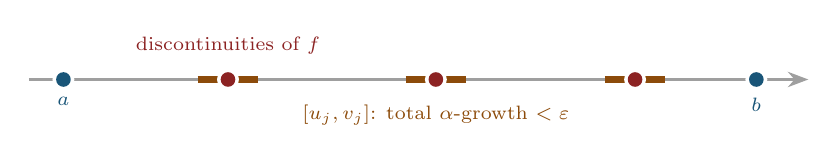
\begin{tikzpicture}[scale=1.1]
    \draw[axisln] (-0.4,0) -- (8.6,0);
    \dotpt{defcolor}{(0,0)}
    \node[defcolor, font=\scriptsize, below=3pt] at (0,0) {$a$};
    \dotpt{defcolor}{(8,0)}
    \node[defcolor, font=\scriptsize, below=3pt] at (8,0) {$b$};
    % bad points with quarantine intervals
    \foreach \x in {1.9, 4.3, 6.6} {
      \draw[excolor, line width=2.6pt] (\x-0.35,0) -- (\x+0.35,0);
      \dotpt{thmcolor}{(\x,0)}
    }
    \node[thmcolor, font=\scriptsize, above] at (1.9,0.18)
      {discontinuities of $f$};
    \node[excolor, font=\scriptsize, below] at (4.3,-0.18)
      {$[u_j, v_j]$: total $\alpha$-growth $< \varepsilon$};
  \end{tikzpicture}
  \end{center}

  \note{
    Let epsilon be given, let capital "M" be the supremum of the
    absolute value of "f", and let "E" be the finite set of points
    where "f" is discontinuous. On the number line, the red dots are
    the bad points, and the orange segments around them are the
    quarantine intervals, "u" sub "j" to "v" sub "j". Because alpha is
    continuous at each bad point, the growth of alpha across a small
    enough interval around that point is as small as we please, so we
    can arrange that the total growth of alpha over all the orange
    intervals is less than epsilon. We also place them so the
    intervals are disjoint and every bad point away from the endpoints
    lies in the interior of the interval that covers it. Now look at what remains.
  }
\end{frame}

\begin{frame}{Proof of Theorem 6.10 --- Step 2: The Good Set Is Compact}
  \begin{proofblock}{Step 2: Uniform continuity off the bad intervals}
    Remove the open segments $(u_j, v_j)$ from $[a,b]$: the remaining set
    $K$ is \alert{compact}, and $f$ is continuous on $K$, hence
    \alert{uniformly continuous}: there is $\delta > 0$ with
    \[
      |f(s) - f(t)| < \varepsilon
      \quad \text{if } s, t \in K,\ |s - t| < \delta.
    \]
  \end{proofblock}

  \note{
    Remove the open quarantine segments from the interval. What
    remains, call it "K", is a closed and bounded subset of the real
    line: closed because we removed open segments from a closed
    interval, bounded trivially. So "K" is compact by the Heine-Borel
    theorem. Every discontinuity of "f" is interior to some removed
    segment, so "f" restricted to "K" is continuous, and continuity
    on a compact set upgrades to uniform continuity, exactly as in
    Theorem 6.8: there is one delta such that values of "f" at points
    of "K" closer than delta differ by less than epsilon. The stage
    is set; now we build the partition.
  }
\end{frame}

\begin{frame}{Proof of Theorem 6.10 --- Step 3: Build $P$ and Estimate}
  \begin{proofblock}{Step 3: The partition}
    Form $P$: every $u_j \in P$, every $v_j \in P$, \alert{no point} of
    any $(u_j, v_j)$ in $P$; if $x_{i-1}$ is not a $u_j$, then
    $\Delta x_i < \delta$. Then
    \[
      M_i - m_i \leq 2M \text{ always}, \qquad
      M_i - m_i \leq \varepsilon \text{ unless } x_{i-1} \text{ is some } u_j.
    \]
    As in Theorem 6.8:
    \[
      U(P,f,\alpha) - L(P,f,\alpha)
      \;\leq\; [\alpha(b) - \alpha(a)]\,\varepsilon + 2M\varepsilon.
    \]
    $\varepsilon$ arbitrary $\Rightarrow$ $f \in \mathscr{R}(\alpha)$
    by Theorem 6.6. \qed
  \end{proofblock}

  \note{
    Build the partition as follows: include every left endpoint "u"
    sub "j" and every right endpoint "v" sub "j" of the quarantine
    intervals, put no points inside them, and chop everything outside
    into pieces shorter than delta. Now estimate the oscillations.
    Every oscillation is at most 2 times capital "M", since all
    values of "f" lie between minus "M" and "M"; this crude bound is
    used on the quarantine subintervals, whose delta alphas add up to
    less than epsilon. Every other subinterval lies in the good set
    "K" and is shorter than delta, so its oscillation is at most
    epsilon; those weights add up to at most the total growth of
    alpha. Adding the two contributions gives the displayed bound:
    the growth of alpha times epsilon, plus 2 "M" epsilon. Since
    epsilon was arbitrary, Theorem 6.6 gives integrability.
  }
\end{frame}

\begin{frame}{A Warning: Shared Jumps Destroy Integrability}
  \begin{remblock}{Note (after Theorem 6.10)}
    If $f$ and $\alpha$ have a \alert{common} point of discontinuity,
    then $f$ need \alert{not} be in $\mathscr{R}(\alpha)$.
    (Exercise 3 shows this.)
  \end{remblock}

  \vspace{0.4em}
  \begin{hlbox}
  \textbf{Moral:} the hypotheses of 6.8--6.10 are a balancing act
  between $f$ and $\alpha$: \alert{at each point, at most one of them may
  jump.}
  \end{hlbox}

  \note{
    A warning closes this circle of ideas. The hypothesis in Theorem
    6.10, that alpha is continuous wherever "f" jumps, is not an
    artifact of the proof. If "f" and alpha jump at the same point,
    integrability can genuinely fail; Exercise 3 of this chapter
    constructs the example, with a step function integrated against
    another step function jumping at the same place. There the upper
    sums and lower sums stay a fixed distance apart no matter how
    fine the partition. The moral is on the slide: the theorems of
    this section are a balancing act between the two players. At any
    given point, at most one of "f" and alpha is allowed to jump.
    One theorem remains, and it is a powerful factory for new
    integrable functions.
  }
\end{frame}

\begin{frame}{Theorem 6.11: Composition with Continuous $\phi$}
  \begin{thmblock}{Theorem 6.11}
    Suppose $f \in \mathscr{R}(\alpha)$ on $[a,b]$, $m \leq f \leq M$,
    $\phi$ is \alert{continuous} on $[m, M]$, and
    $h(x) = \phi(f(x))$ on $[a,b]$.
    Then $h \in \mathscr{R}(\alpha)$ on $[a,b]$.
  \end{thmblock}

  \vspace{0.4em}
  \begin{hlbox}
  \textbf{Examples to come:} $\phi(t) = t^2$ and $\phi(t) = |t|$ \
  $\Rightarrow$ \ $f^2$, $|f| \in \mathscr{R}(\alpha)$ \
  (used to prove $fg \in \mathscr{R}(\alpha)$ in the next section).
  \end{hlbox}

  \note{
    The last theorem of the section, Theorem 6.11, is a machine for
    producing new integrable functions from old ones. Suppose "f" is
    integrable with respect to alpha and its values lie in the closed
    interval from "m" to capital "M". Let phi be any continuous
    function on that interval, and let "h" be the composition, "h" of
    "x" equals phi of "f" of "x". The claim: "h" is integrable too.
    The examples on the slide show why we care: taking phi of "t"
    equal to "t" squared shows the square of an integrable function
    is integrable, and phi of "t" equal to the absolute value of "t"
    handles absolute values; in the next section these two facts
    yield that products of integrable functions are integrable. The
    proof is the most delicate of the section, so let's first fix
    the strategy.
  }
\end{frame}

\begin{frame}{Proof of Theorem 6.11 --- Strategy}
  \begin{hlbox}
  \textbf{Goal:} make $U(P,h,\alpha) - L(P,h,\alpha)$ small, knowing
  that this works for $f$.

  \vspace{0.5em}
  \textbf{Approach:}
  \begin{enumerate}
    \item $\phi$ is \alert{uniformly continuous}: small input gaps
      $\Rightarrow$ small output gaps
    \item Take $P$ with $U(P,f,\alpha) - L(P,f,\alpha) < \delta^2$
      \ (note: $\delta$ \alert{squared}!)
    \item Split indices: class $A$ (small oscillation of $f$),
      class $B$ (large oscillation)
    \item On $A$: $\phi$ keeps oscillations small.
      On $B$: oscillation $\leq 2K$, but $B$ carries
      \alert{little $\alpha$-weight}
  \end{enumerate}
  \end{hlbox}

  \note{
    Here is the plan. We must verify the criterion for "h", knowing it
    for "f". First, phi is continuous on a compact interval, hence
    uniformly continuous: a delta controls how much phi can spread
    values. Second, and this is the clever move, we choose a partition
    for "f" whose gap "U" minus "L" is less than delta squared, not
    just delta; keep an eye on that exponent. Third, we sort the
    subintervals into two classes: class "A", where "f" oscillates
    less than delta, and class "B", where it oscillates by delta or
    more. On class "A" subintervals, uniform continuity of phi keeps
    the oscillation of "h" small. On class "B" we only have a crude
    bound, but the delta squared budget will force the total alpha
    weight of class "B" to be tiny. Let's execute.
  }
\end{frame}

\begin{frame}{Proof of Theorem 6.11 --- Step 1: Calibrate and Partition}
  \begin{proofblock}{Step 1: Choices}
    Choose $\varepsilon > 0$. Uniform continuity of $\phi$ on $[m,M]$
    gives $\delta > 0$ with $\delta < \varepsilon$ and
    \[
      |\phi(s) - \phi(t)| < \varepsilon
      \quad \text{if } |s - t| \leq \delta, \quad s, t \in [m, M].
    \]
    Since $f \in \mathscr{R}(\alpha)$, there is a partition $P$ with
    \begin{equation}
      U(P,f,\alpha) - L(P,f,\alpha) < \delta^2. \tag{18}
    \end{equation}
  \end{proofblock}

  \note{
    Choose epsilon. Since phi is continuous on the compact interval
    from "m" to capital "M", it is uniformly continuous there, so
    there is a delta, which we may also take smaller than epsilon,
    such that whenever two inputs differ by at most delta, the
    outputs of phi differ by less than epsilon. Since "f" is
    integrable, Theorem 6.6 provides a partition "P" satisfying
    inequality 18: the gap for "f" is less than delta squared. We are
    entitled to demand delta squared instead of epsilon because the
    criterion works for every positive tolerance, and delta squared
    is just another positive number. Now the class division.
  }
\end{frame}

\begin{frame}{Proof of Theorem 6.11 --- Step 2: Two Classes}
  \begin{proofblock}{Step 2: Classes $A$ and $B$}
    Let $M_i^*$, $m_i^*$ be the sup/inf of $h$ (with $M_i$, $m_i$ those
    of $f$). Divide $1, \dots, n$:
    \[
      i \in A \ \text{ if } M_i - m_i < \delta, \qquad
      i \in B \ \text{ if } M_i - m_i \geq \delta.
    \]
    \begin{itemize}
      \item $i \in A$: \ $M_i^* - m_i^* \leq \varepsilon$
        \ (choice of $\delta$)
      \item $i \in B$: \ $M_i^* - m_i^* \leq 2K$, \
        where $K = \sup_{[m,M]} |\phi(t)|$
    \end{itemize}
  \end{proofblock}

  \note{
    Write "M" sub "i" star and "m" sub "i" star for the supremum and
    infimum of "h" on subinterval number "i", keeping the unstarred
    letters for "f". Sort the indices: "i" goes to class "A" if the
    oscillation of "f" there is less than delta, and to class "B" if
    it is at least delta. On a class "A" subinterval, any two values
    of "f" differ by less than delta, so by our choice of delta, the
    corresponding values of "h", which are phi applied to values of
    "f", differ by less than epsilon; hence the oscillation of "h" is
    at most epsilon. On a class "B" subinterval we settle for the
    trivial bound: all values of "h" lie between minus "K" and "K",
    where "K" is the supremum of the absolute value of phi, so the
    oscillation is at most 2 "K". The next step shows class "B" is
    small in the only sense that matters.
  }
\end{frame}

\begin{frame}{Proof of Theorem 6.11 --- Step 3: Class $B$ Has Small Weight}
  \begin{proofblock}{Step 3: The $\delta^2$ trick}
    By (18),
    \begin{equation}
      \delta \sum_{i \in B} \Delta\alpha_i
      \;\leq\; \sum_{i \in B} (M_i - m_i)\,\Delta\alpha_i
      \;<\; \delta^2, \tag{19}
    \end{equation}
    so that
    \[
      \boxed{\ \sum_{i \in B} \Delta\alpha_i < \delta\ }
    \]
  \end{proofblock}

  \vspace{0.3em}
  \begin{hlbox}
  \textbf{The point of $\delta^2$:} one $\delta$ pays for the
  \alert{height} $2K$, the other for the \alert{width}.
  \end{hlbox}

  \note{
    Here is where delta squared pays off. On each class "B"
    subinterval the oscillation of "f" is at least delta, by the very
    definition of class "B". So delta times the total alpha weight of
    class "B" is at most the sum over "B" of oscillation times
    weight, which is at most the full sum "U" minus "L", and that is
    less than delta squared by inequality 18. This is inequality 19.
    Dividing by delta, the boxed conclusion appears: the total alpha
    weight of the bad class is less than delta. This is the same
    style of argument as the Chebyshev inequality in probability:
    where the oscillation is large, the weight must be small, or the
    total budget would be exceeded. As the last line says, one
    factor of delta pays for the height of the bad rectangles, the
    other for their width. Now we assemble the estimate.
  }
\end{frame}

\begin{frame}{Proof of Theorem 6.11 --- Step 4: Assemble}
  \begin{proofblock}{Step 4: Conclusion}
    \begin{align*}
      U(P,h,\alpha) - L(P,h,\alpha)
      &= \sum_{i \in A} (M_i^* - m_i^*)\,\Delta\alpha_i
        + \sum_{i \in B} (M_i^* - m_i^*)\,\Delta\alpha_i \\
      &\leq \varepsilon\,[\alpha(b) - \alpha(a)] + 2K\delta
        \;<\; \varepsilon\,[\alpha(b) - \alpha(a) + 2K].
    \end{align*}
    $\varepsilon$ arbitrary $\Rightarrow$ $h \in \mathscr{R}(\alpha)$
    by Theorem 6.6. \qed
  \end{proofblock}

  \note{
    Split "U" minus "L" for "h" into the class "A" part and the class
    "B" part. Over class "A", each oscillation of "h" is at most
    epsilon, and the weights add up to at most the total growth of
    alpha; that gives the first term. Over class "B", each
    oscillation is at most 2 "K", and by the boxed estimate the
    weights add up to less than delta; that gives the second term, 2
    "K" delta. Finally, recall we arranged delta less than epsilon,
    so the whole bound is less than epsilon times the bracketed
    constant: the growth of alpha plus 2 "K". That constant is fixed,
    and epsilon was arbitrary, so the criterion of Theorem 6.6 is
    met, and "h" is integrable. Composition with a continuous
    function preserves integrability.
  }
\end{frame}

\begin{frame}{Remark: Just \emph{Which} Functions Are Integrable?}
  \begin{remblock}{Remark (after Theorem 6.11)}
    Theorem 6.11 suggests the question: \alert{just what functions are
    Riemann-integrable?} The complete answer comes much later, in
    Theorem 11.33(b) (Lebesgue's criterion).
  \end{remblock}

  \vspace{0.4em}
  \begin{hlbox}
  \textbf{Spoiler:} $f \in \mathscr{R}$ $\iff$ $f$ is bounded and
  continuous \alert{almost everywhere} --- but ``almost everywhere''
  needs \emph{measure theory} (Chapter 11).
  \end{hlbox}

  \note{
    We close the theory with the natural question raised by this
    string of results: exactly which functions are Riemann
    integrable? We have sufficient conditions, continuity,
    monotonicity, finitely many discontinuities, compositions, but no
    exact characterization. Rudin points ahead to Theorem 11.33 part
    "b", at the very end of the book. The answer, due to Lebesgue,
    is remarkably clean: a bounded function is Riemann integrable if
    and only if its set of discontinuities is negligible in a precise
    sense, namely has measure zero. Making sense of that requires
    the measure theory of Chapter 11, so for now we treat it as a
    preview of coming attractions. Let's summarize the episode.
  }
\end{frame}

}

{
\usebackgroundtemplate{%
  
\includegraphics[width=\paperwidth,height=\paperheight,keepaspectratio=false]{chapter_06_bg_07.png}%
}
\section{Summary}

% --- Build 1/3 ---
\begin{frame}{Summary}
  \begin{hlbox}
  \textbf{Key takeaways from this section:}
  \footnotesize
  \begin{itemize}
    \item \textbf{Two definitions:} upper/lower sums define
      $\overline{\int} f\,dx \geq \underline{\int} f\,dx$; equality $=$
      \alert{integrability}. With $\Delta\alpha_i$ for $\Delta x_i$:
      the \alert{Riemann--Stieltjes} integral $\int f\,d\alpha$
  \end{itemize}
  \end{hlbox}

  \note{
    Let's review what we covered. First, the definitions. A partition
    chops the interval into finitely many pieces; the supremum and
    infimum of "f" on each piece generate the upper and lower sums,
    and optimizing
    over all partitions gives the upper and lower integrals, which
    always exist for bounded "f" and always sit in the right order.
    Integrability means they coincide. And the same construction with
    the length delta "x" sub "i" replaced by the growth delta alpha
    sub "i" of an increasing weight function defines the
    Riemann-Stieltjes integral; choosing alpha of "x" equal to "x"
    recovers the ordinary Riemann integral as a special case.
  }
\end{frame}

% --- Build 2/3 ---
\begin{frame}{Summary}
  \begin{hlbox}
  \textbf{Key takeaways from this section:}
  \footnotesize
  \begin{itemize}
    \item \textbf{Two definitions:} upper/lower sums define
      $\overline{\int} f\,dx \geq \underline{\int} f\,dx$; equality $=$
      \alert{integrability}. With $\Delta\alpha_i$ for $\Delta x_i$:
      the \alert{Riemann--Stieltjes} integral $\int f\,d\alpha$
    \item \textbf{The machinery:} refinements tighten the trap (6.4),
      so $\underline{\int} \leq \overline{\int}$ (6.5);\\
      \alert{Theorem 6.6}: $f \in \mathscr{R}(\alpha) \iff$
      $U - L < \varepsilon$ for some $P$;\\
      Riemann sums then approximate the integral (6.7)
  \end{itemize}
  \end{hlbox}

  \note{
    Second, the machinery. Theorem 6.4: refining a partition raises
    lower sums and lowers upper sums, so the trap only tightens; via
    the common refinement this gave Theorem 6.5, the lower integral
    never exceeds the upper one. The workhorse is Theorem 6.6, the
    Cauchy-style criterion: integrability is equivalent to finding,
    for each epsilon, a single partition whose upper and lower sums
    differ by less than epsilon. Theorem 6.7 added the practical
    consequences: good partitions stay good under refinement, and
    Riemann-Stieltjes sums built from arbitrary sample points
    approximate the integral to within epsilon.
  }
\end{frame}

% --- Build 3/3 ---
\begin{frame}{Summary}
  \begin{hlbox}
  \textbf{Key takeaways from this section:}
  \footnotesize
  \begin{itemize}
    \item \textbf{Two definitions:} upper/lower sums define
      $\overline{\int} f\,dx \geq \underline{\int} f\,dx$; equality $=$
      \alert{integrability}. With $\Delta\alpha_i$ for $\Delta x_i$:
      the \alert{Riemann--Stieltjes} integral $\int f\,d\alpha$
    \item \textbf{The machinery:} refinements tighten the trap (6.4),
      so $\underline{\int} \leq \overline{\int}$ (6.5);\\
      \alert{Theorem 6.6}: $f \in \mathscr{R}(\alpha) \iff$
      $U - L < \varepsilon$ for some $P$;\\
      Riemann sums then approximate the integral (6.7)
    \item \textbf{Who is integrable:} $f$ continuous (6.8); $f$
      monotonic $+$ $\alpha$ continuous (6.9); finitely many
      discontinuities avoiding those of $\alpha$ (6.10);
      $\phi \circ f$, $\phi$ continuous (6.11)
  \end{itemize}

  \textbf{Coming up next:} Properties of the Integral --- linearity,
  products, \alert{series as integrals}.
  \end{hlbox}

  \note{
    Third, the harvest: who is integrable. Continuous functions
    always are, by uniform continuity, Theorem 6.8. Monotonic
    functions are, provided alpha is continuous, Theorem 6.9. Bounded
    functions with finitely many discontinuities are, provided alpha
    is continuous at each of those points, Theorem 6.10, and we saw
    that shared jumps genuinely destroy integrability. Finally,
    Theorem 6.11: composing an integrable function with a continuous
    one preserves integrability, the delta squared argument. In the
    next episode we develop the properties of the integral:
    linearity, behavior under products and absolute values, splitting
    the interval, and the beautiful step-function weights that make
    an infinite series literally a Stieltjes integral. See you there.
  }
\end{frame}
}

\end{document}
